% ============================================================
% SECTION 3 - UI/UX THIẾT KẾ
% Kiến trúc thông tin · First Run · Luồng C1 · Mockup
% Design System · Typography · Component · Accessibility
% Micro-interactions
% ============================================================
\section{UI/UX thiết kế}

% ------------------------------------------------------------
\subsection{Kiến trúc thông tin: Cấu trúc và điều hướng}
% ------------------------------------------------------------
\begin{frame}{Kiến trúc thông tin --- Cấu trúc và điều hướng}
\begin{columns}[T]
\begin{column}{0.50\textwidth}
\footnotesize
\textbf{IA tổ chức nội dung để người dùng điều hướng tự nhiên}
\vspace{2mm}
{\tiny
\begin{itemize}\setlength{\itemsep}{4pt}
\item \textbf{Cấu trúc phân cấp:} \newline Thanh tab chính $\rightarrow$ danh mục $\rightarrow$ màn chi tiết
\item \textbf{Bottom Navigation:} \newline 5 tab (Home -- Video -- Music -- News -- Games); đây là điều hướng chính
\item \textbf{Bottom Sheet / Dialog:} \newline tác vụ tạm (xác nhận đăng xuất, chọn khung avatar, xem sau, hàng đợi nhạc)
\item \textbf{Không dùng Navigation Drawer:} \newline tần suất thấp; che gần nửa màn hình
\end{itemize}}
\end{column}
\begin{column}{0.46\textwidth}
\centering
\begin{tikzpicture}[scale=0.75]
  \node[draw=BKTemplate!60, rounded corners=3pt, fill=BKTemplate!8, font=\tiny\bfseries, minimum width=2.4cm] (nav) at (0,0) {Thanh tab chính (5)};
  \node[draw=BKTemplate!60, rounded corners=2pt, fill=BKTemplate!5, font=\tiny, minimum width=0.85cm] (home) at (-3.1,-1.0) {Home};
  \node[draw=BKTemplate!60, rounded corners=2pt, fill=BKTemplate!5, font=\tiny, minimum width=0.85cm] (video) at (-1.55,-1.0) {Video};
  \node[draw=BKTemplate!60, rounded corners=2pt, fill=BKTemplate!5, font=\tiny, minimum width=0.85cm] (music) at (0,-1.0) {Music};
  \node[draw=BKTemplate!60, rounded corners=2pt, fill=BKTemplate!5, font=\tiny, minimum width=0.85cm] (news) at (1.55,-1.0) {News};
  \node[draw=TextGray!40, rounded corners=2pt, fill=TextGray!5, font=\tiny, minimum width=0.85cm] (games) at (3.1,-1.0) {Games};
  \draw[-{Latex}, BKTemplate!50] (nav) -- (home);
  \draw[-{Latex}, BKTemplate!50] (nav) -- (video);
  \draw[-{Latex}, BKTemplate!50] (nav) -- (music);
  \draw[-{Latex}, BKTemplate!50] (nav) -- (news);
  \draw[-{Latex}, TextGray!50] (nav) -- (games);
  \node[draw=TextGray!40, rounded corners=2pt, fill=TextGray!5, font=\tiny, text width=1.2cm, align=center] (detail) at (-2.4,-2.6) {Màn chi tiết};
  \node[draw=TextGray!40, rounded corners=2pt, fill=TextGray!5, font=\tiny, text width=1.2cm, align=center] (play) at (2.4,-2.6) {Màn chơi};
  \draw[-{Latex}, TextGray!50] (home.south) -- ++(0,-0.33) -| (detail.north);
  \draw[-{Latex}, TextGray!50] (games.south) -- ++(0,-0.33) -| (play.north);
  \node[font=\tiny, text=TextGray] at (0,-1.75) {\textit{danh mục / feed}};
\end{tikzpicture}
\end{column}
\end{columns}
\end{frame}

% ------------------------------------------------------------
\subsection{Kiến trúc thông tin: Tìm kiếm và bố cục}
% ------------------------------------------------------------
\begin{frame}{Kiến trúc thông tin --- Tìm kiếm và bố cục}
\small
\begin{itemize}\setlength{\itemsep}{4pt}
\item \textbf{Tìm kiếm và lọc:} ô tìm trên Home gợi ý cả bốn phân hệ (F-COM-11); mỗi phân hệ có ô tìm riêng (tiêu đề, nghệ sĩ, bài báo)
\item \textbf{Một màn một hành động chính;} chi tiết giấu theo cấp độ (progressive disclosure): menu cài đặt phát chỉ mở khi bấm bánh răng, khối quiz chỉ hiện khi bấm ``Chơi nhanh''
\item Trạng thái (bài đang phát, video nổi, ván dở) đi theo người dùng khi đổi tab~--~chuyển phân hệ không làm mất ngữ cảnh
\end{itemize}
\end{frame}

% ------------------------------------------------------------
\subsection{Trải nghiệm đầu tiên (First Run)}
% ------------------------------------------------------------
\begin{frame}{Trải nghiệm đầu tiên (First Run) --- Luồng 8 bước}
\begin{center}
\begin{tikzpicture}[
    stp/.style={circle, draw=BKTemplate, thick, fill=BKTemplate!12, minimum size=0.72cm, font=\small\bfseries, text=BKTemplate},
    desc/.style={text width=2.75cm, align=center, font=\tiny}]
  \node[stp] (s1) at (0.9,4.1) {1};
  \node[desc, below=0.12cm of s1] {Mở app $\leq$ 2 giây, không bắt đăng nhập};
  \node[stp] (s2) at (4.5,4.1) {2};
  \node[desc, below=0.12cm of s2] {Chọn $\geq$ 3 chủ đề (bỏ qua được)};
  \node[stp] (s3) at (8.1,4.1) {3};
  \node[desc, below=0.12cm of s3] {Home hiện ``Đề xuất hôm nay'': 1 video, 1 bài hát, 1 tin};
  \node[stp] (s4) at (11.7,4.1) {4};
  \node[desc, below=0.12cm of s4] {Chạm bài hát $\rightarrow$ dock mini hiện ở đáy};
  \node[stp] (s5) at (11.7,1.5) {5};
  \node[desc, below=0.12cm of s5] {Banner nhiệm vụ: nghe 1 bài -- đọc 1 tin -- thắng 1 ván};
  \node[stp] (s6) at (8.1,1.5) {6};
  \node[desc, below=0.12cm of s6] {Mở bài tin: dock nhạc vẫn hiện trong trình đọc};
  \node[stp] (s7) at (4.5,1.5) {7};
  \node[desc, below=0.12cm of s7] {Hoàn 3 nhiệm vụ $\rightarrow$ trứng thú cưng nở};
  \node[stp] (s8) at (0.9,1.5) {8};
  \node[desc, below=0.12cm of s8] {Cuối phiên: streak = 1, huy hiệu ``Chuỗi 7 ngày''};
  \draw[-{Latex}, BKTemplate!60] (s1) -- (s2);
  \draw[-{Latex}, BKTemplate!60] (s2) -- (s3);
  \draw[-{Latex}, BKTemplate!60] (s3) -- (s4);
  \draw[-{Latex}, BKTemplate!60] (s4.east) -- ++(0.85,0) |- (s5.east);
  \draw[-{Latex}, BKTemplate!60] (s5) -- (s6);
  \draw[-{Latex}, BKTemplate!60] (s6) -- (s7);
  \draw[-{Latex}, BKTemplate!60] (s7) -- (s8);
\end{tikzpicture}
\end{center}
\vfill
{\small\textbf{Onboarding theo 3 nguyên tắc}}\vspace{1mm}
{\small
\begin{itemize}\setlength{\itemsep}{3pt}
\item \textbf{Giá trị:} ba màn đầu nói rõ app giải quyết được gì cho người dùng
\item \textbf{Quyền riêng tư:} không xin quyền ngay lúc mở app
\item \textbf{Liền mạch:} không bắt đăng nhập trước khi thấy được sản phẩm
\end{itemize}}
\end{frame}

% ------------------------------------------------------------
\subsection{Luồng xử lý xung đột âm thanh (C1)}
% ------------------------------------------------------------
\begin{frame}{Luồng xử lý xung đột âm thanh (C1)}
\begin{center}
\begin{tikzpicture}[
    font=\scriptsize,
    stp/.style={draw=BKTemplate, thick, rounded corners=3.5pt, fill=BKTemplate!8, minimum height=8mm, align=center, text width=2.6cm},
    term/.style={draw=BKTemplate, thick, rounded corners=4mm, fill=BKTemplate!20, minimum height=6mm, align=center, inner sep=2.5pt},
    dec/.style={diamond, aspect=1.9, draw=BKTemplate, thick, fill=BKTemplate!12, align=center, inner sep=1pt},
    lnk/.style={draw=black!50, -{Latex[length=1.6mm]}}]
  \node[stp] (v) at (0,0) {Video đang phát};
  \node[term, above=0.5cm of v] (st) {Bắt đầu};
  \node[stp, right=0.7cm of v] (m) {Người dùng mở bài nhạc};
  \node[dec, right=0.7cm of m] (q) {Đã lưu quy tắc?};
  \node[stp, right=0.7cm of q] (r) {Áp dụng im lặng};
  \node[stp, below=1.05cm of q] (p) {Popup 2 lựa chọn + ô tick};
  \node[stp, below=1.05cm of p] (s) {Tick: ghi nhớ đúng lựa chọn này};
  \node[term, below=1.6cm of r] (en) {Kết thúc};
  \draw[lnk] (st) -- (v);
  \draw[lnk] (v) -- (m);
  \draw[lnk] (m) -- (q);
  \draw[lnk] (q) -- node[above, font=\tiny]{Có} (r);
  \draw[lnk] (q.south) -- node[right, font=\tiny]{Không} ++(0,-0.45) -| (p.north);
  \draw[lnk] (p.south) -- ++(0,-0.45) -| (s.north);
  \draw[lnk] (r.south) -- (en.north);
  \draw[lnk] (s.east) -- (en.west);
\end{tikzpicture}
\end{center}
\vfill
{\tiny\color{TextGray} Tích ``Không hỏi lại'' để ghi nhớ; đặt lại ``Luôn hỏi'' trong Cài đặt (F-COM-14, popup 2 lựa chọn).}
\end{frame}

% ------------------------------------------------------------
\subsection{Mock up}
% ------------------------------------------------------------
\begin{frame}{Mock up --- ảnh chụp từ app chạy thật}
\begin{columns}[T]
\begin{column}{0.55\textwidth}
\footnotesize
\begin{itemize}\setlength{\itemsep}{4pt}
\item \textbf{74 mã tính năng} đều có ảnh chụp thật từ app chạy trên emulator
\item Ảnh xếp theo phân hệ: Video $\rightarrow$ Nhạc $\rightarrow$ Tin tức $\rightarrow$ Trò chơi $\rightarrow$ Dùng chung
\item Tính năng có nhiều màn hình thì chia slide, mỗi slide 2 ảnh
\end{itemize}
\end{column}
\begin{column}{0.41\textwidth}
\begin{exampleblock}{\scriptsize\bfseries Prototype}
{\tiny Mockup trong bài là \textbf{ảnh chụp từ app chạy được}~--~demo trực tiếp trên emulator.\\[1mm]
Mọi feed xử lý đủ 4 trạng thái: đang tải (skeleton) $\cdot$ lỗi $\cdot$ trống $\cdot$ có dữ liệu.}
\end{exampleblock}
\end{column}
\end{columns}
\end{frame}

% ===== MOCKUP SECTION (sinh bởi scripts/gen_mockups.py — chạy lại sau khi thêm ảnh) =====


\begin{frame}{Mock Up: Phân hệ Video}
\begin{columns}[T]
\begin{column}{0.46\textwidth}
{\small\bfseries\color{BKTemplate} F-VID-01: Xem video streaming cơ bản (player HLS/MP4)}\\[2.5mm]
Tính năng thuộc nhóm Major Projects
\end{column}
\begin{column}{0.50\textwidth}
\centering
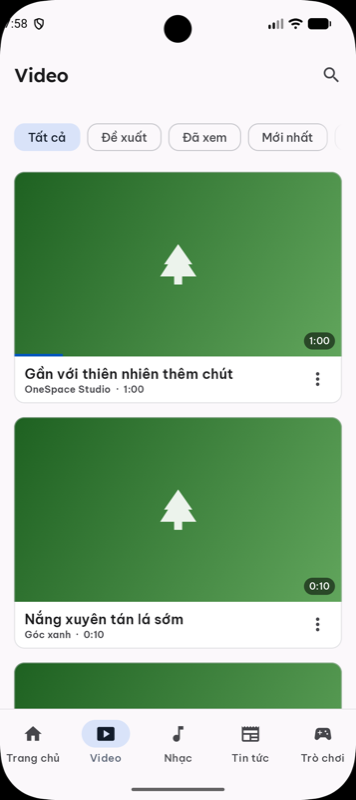
\includegraphics[width=2.75cm]{../figures/app/F-VID-01-01.png}\hspace{0.25cm}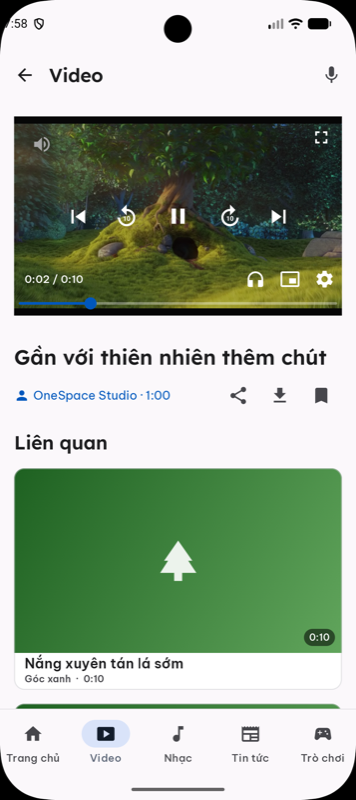
\includegraphics[width=2.75cm]{../figures/app/F-VID-01-02.png}
\end{column}
\end{columns}
\end{frame}

\begin{frame}{Mock Up: Phân hệ Video}
\begin{columns}[T]
\begin{column}{0.46\textwidth}
{\small\bfseries\color{BKTemplate} F-VID-02: Feed ``Đề xuất'' theo sở thích}\\[2.5mm]
Tính năng thuộc nhóm Major Projects
\end{column}
\begin{column}{0.50\textwidth}
\centering
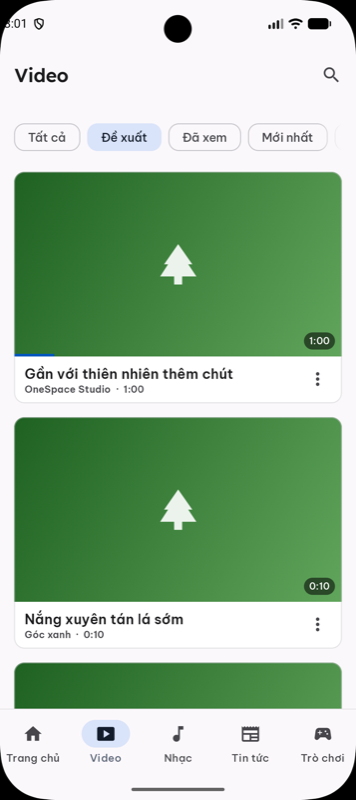
\includegraphics[height=6.1cm]{../figures/app/F-VID-02-01.png}
\end{column}
\end{columns}
\end{frame}

\begin{frame}{Mock Up: Phân hệ Video}
\begin{columns}[T]
\begin{column}{0.46\textwidth}
{\small\bfseries\color{BKTemplate} F-VID-03: Tìm kiếm video}\\[2.5mm]
Tính năng thuộc nhóm Quick Wins
\end{column}
\begin{column}{0.50\textwidth}
\centering
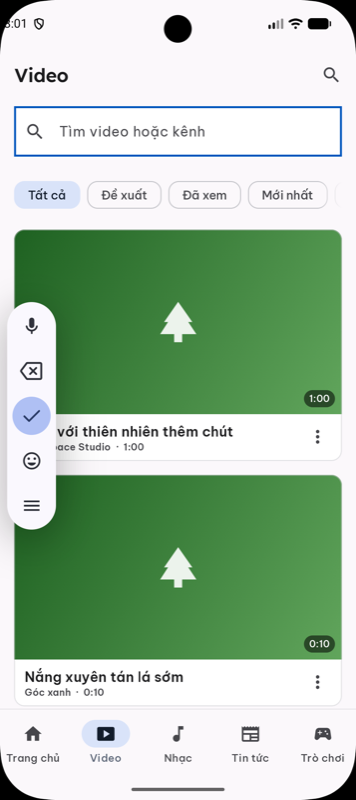
\includegraphics[width=2.75cm]{../figures/app/F-VID-03-01.png}\hspace{0.25cm}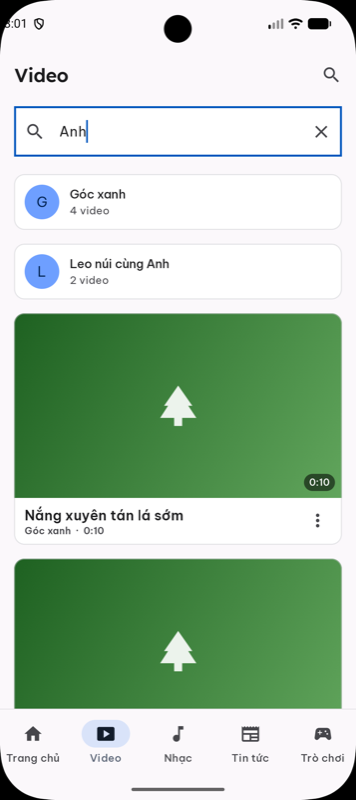
\includegraphics[width=2.75cm]{../figures/app/F-VID-03-02.png}
\end{column}
\end{columns}
\end{frame}

\begin{frame}{Mock Up: Phân hệ Video}
\begin{columns}[T]
\begin{column}{0.46\textwidth}
{\small\bfseries\color{BKTemplate} F-VID-04: Danh sách xem sau (watchlist)}\\[2.5mm]
Tính năng thuộc nhóm Quick Wins
\end{column}
\begin{column}{0.50\textwidth}
\centering
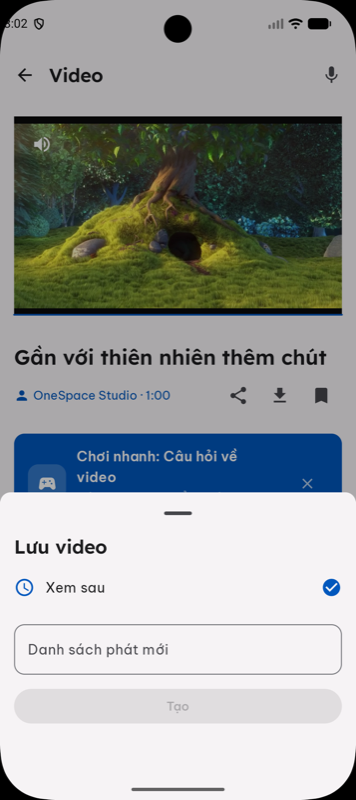
\includegraphics[width=2.75cm]{../figures/app/F-VID-04-01.png}\hspace{0.25cm}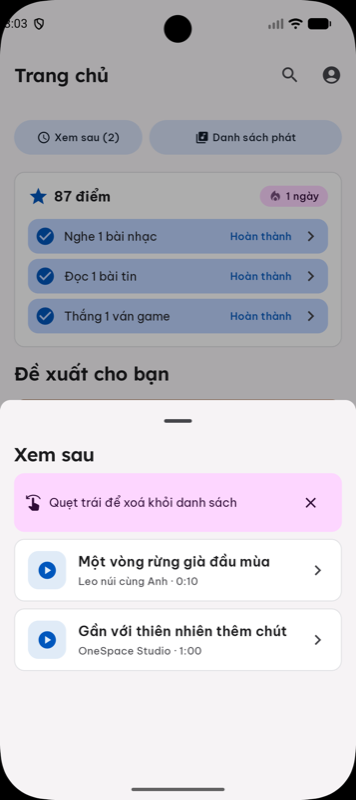
\includegraphics[width=2.75cm]{../figures/app/F-VID-04-02.png}
\end{column}
\end{columns}
\end{frame}

\begin{frame}{Mock Up: Phân hệ Video}
\begin{columns}[T]
\begin{column}{0.46\textwidth}
{\small\bfseries\color{BKTemplate} F-VID-05: Lịch sử xem và tiếp tục từ chỗ dừng}\\[2.5mm]
Tính năng thuộc nhóm Quick Wins
\end{column}
\begin{column}{0.50\textwidth}
\centering
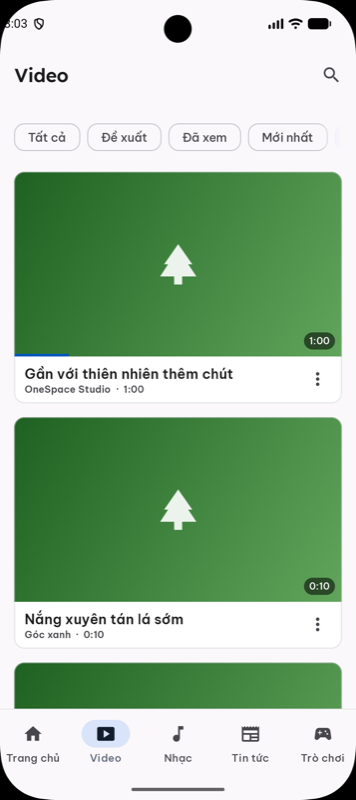
\includegraphics[height=6.1cm]{../figures/app/F-VID-05-01.png}
\end{column}
\end{columns}
\end{frame}

\begin{frame}{Mock Up: Phân hệ Video}
\begin{columns}[T]
\begin{column}{0.46\textwidth}
{\small\bfseries\color{BKTemplate} F-VID-06: Chọn chất lượng phát: Auto hoặc bản 1080p/720p/360p}\\[2.5mm]
Tính năng thuộc nhóm Major Projects
\end{column}
\begin{column}{0.50\textwidth}
\centering
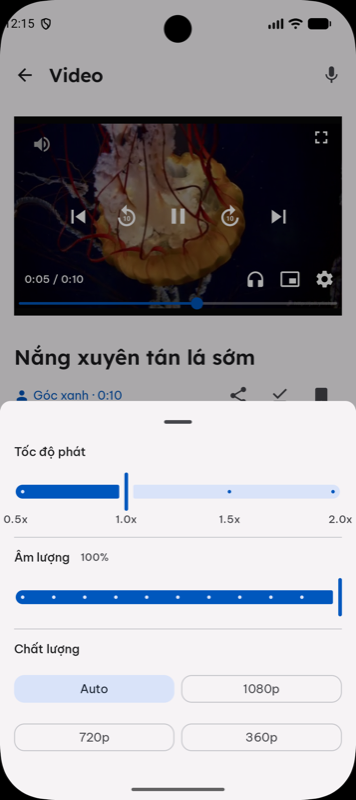
\includegraphics[height=6.1cm]{../figures/app/F-VID-06-01.png}
\end{column}
\end{columns}
\end{frame}

\begin{frame}{Mock Up: Phân hệ Video}
\begin{columns}[T]
\begin{column}{0.46\textwidth}
{\small\bfseries\color{BKTemplate} F-VID-07: Tải video xem offline}\\[2.5mm]
Tính năng thuộc nhóm Thankless
\end{column}
\begin{column}{0.50\textwidth}
\centering
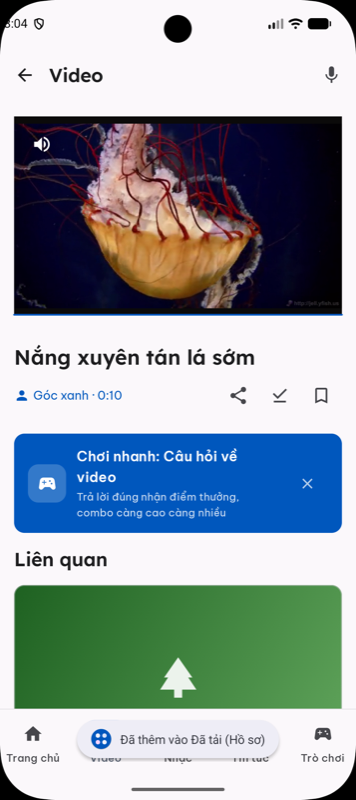
\includegraphics[width=2.32cm]{../figures/app/F-VID-07-01.png}\hspace{0.2cm}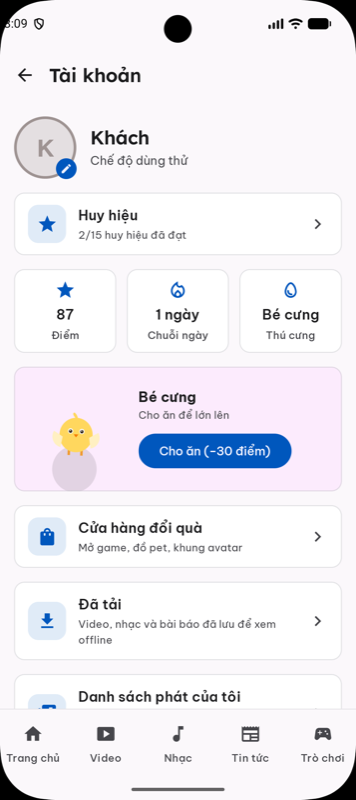
\includegraphics[width=2.32cm]{../figures/app/F-VID-07-02.png}\hspace{0.2cm}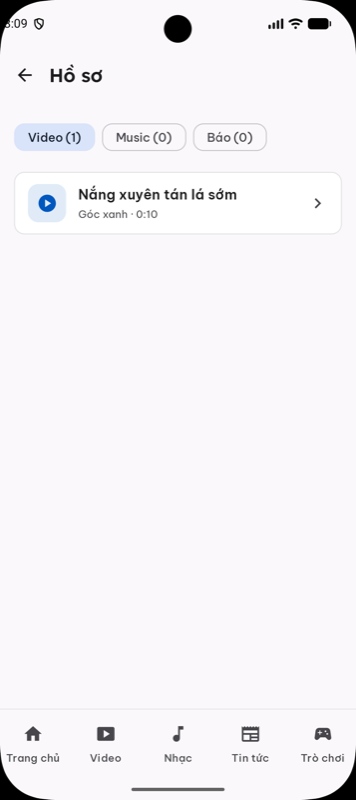
\includegraphics[width=2.32cm]{../figures/app/F-VID-07-03.png}
\end{column}
\end{columns}
\end{frame}

\begin{frame}{Mock Up: Phân hệ Video}
\begin{columns}[T]
\begin{column}{0.46\textwidth}
{\small\bfseries\color{BKTemplate} F-VID-08: Picture-in-picture: video thu nhỏ góc màn hình khi rời trang}\\[2.5mm]
Tính năng thuộc nhóm Major Projects
\end{column}
\begin{column}{0.50\textwidth}
\centering
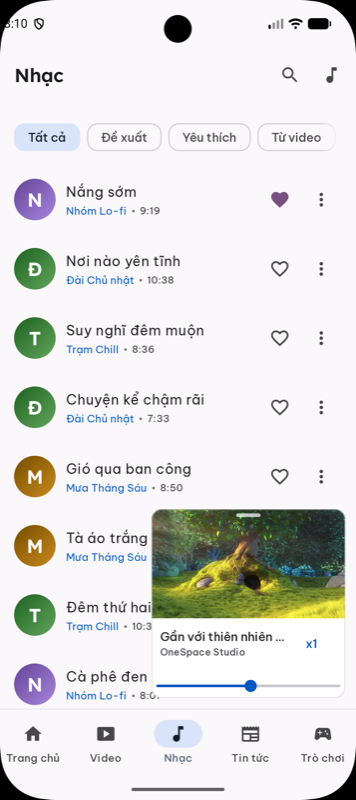
\includegraphics[height=6.1cm]{../figures/app/F-VID-08-01.png}
\end{column}
\end{columns}
\end{frame}

\begin{frame}{Mock Up: Phân hệ Video}
\begin{columns}[T]
\begin{column}{0.46\textwidth}
{\small\bfseries\color{BKTemplate} F-VID-09: Chế độ chỉ phát âm thanh của video (audio-only)}\\[2.5mm]
Tính năng thuộc nhóm Fill-ins
\end{column}
\begin{column}{0.50\textwidth}
\centering
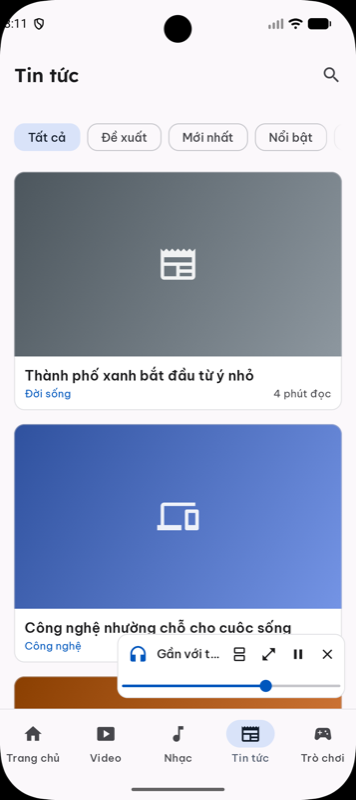
\includegraphics[height=6.1cm]{../figures/app/F-VID-09-01.png}
\end{column}
\end{columns}
\end{frame}

\begin{frame}{Mock Up: Phân hệ Video}
\begin{columns}[T]
\begin{column}{0.46\textwidth}
{\small\bfseries\color{BKTemplate} F-VID-10: Nhấn giữ video để trích thành tệp mp3 cho kho cá nhân}\\[2.5mm]
Tính năng thuộc nhóm Major Projects
\end{column}
\begin{column}{0.50\textwidth}
\centering
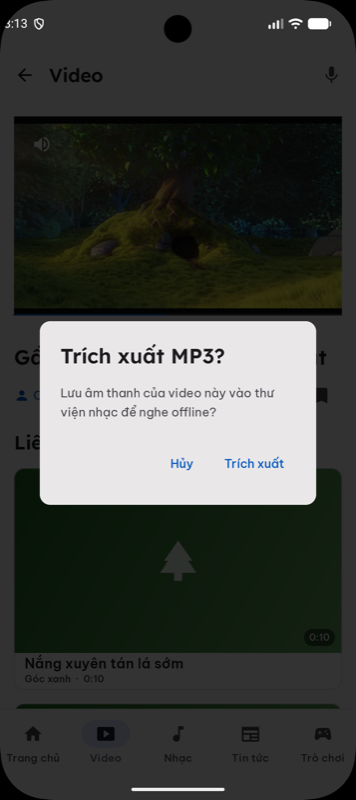
\includegraphics[width=2.32cm]{../figures/app/F-VID-10-01.png}\hspace{0.2cm}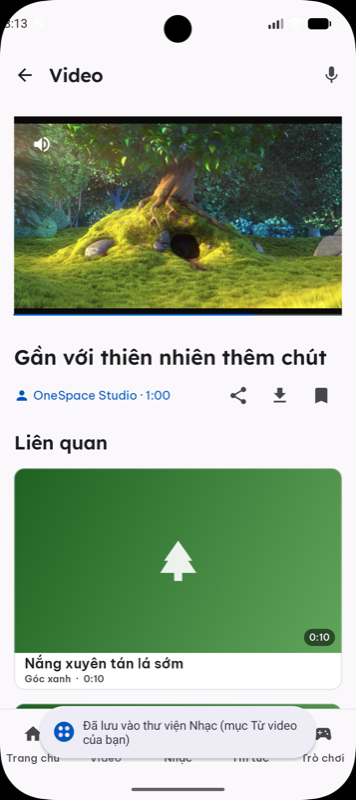
\includegraphics[width=2.32cm]{../figures/app/F-VID-10-02.png}\hspace{0.2cm}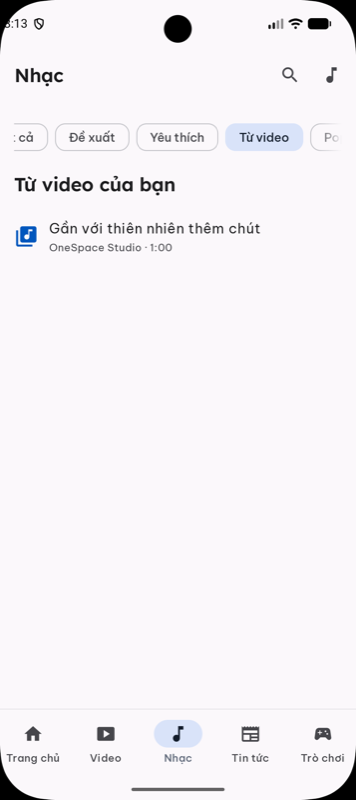
\includegraphics[width=2.32cm]{../figures/app/F-VID-10-03.png}
\end{column}
\end{columns}
\end{frame}

\begin{frame}{Mock Up: Phân hệ Video}
\begin{columns}[T]
\begin{column}{0.46\textwidth}
{\small\bfseries\color{BKTemplate} F-VID-11: Chia sẻ link video ra ngoài app}\\[2.5mm]
Tính năng thuộc nhóm Fill-ins
\end{column}
\begin{column}{0.50\textwidth}
\centering
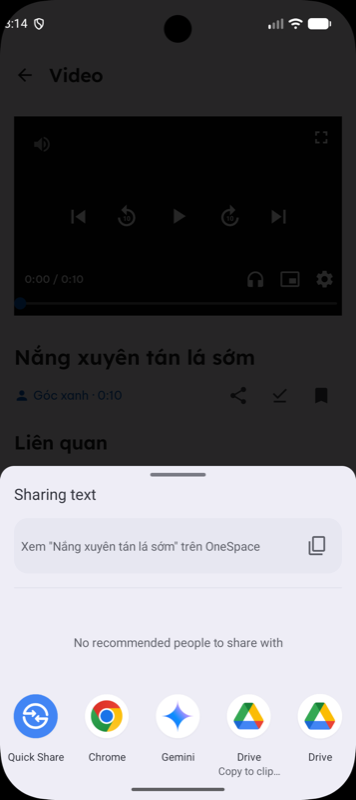
\includegraphics[height=6.1cm]{../figures/app/F-VID-11-01.png}
\end{column}
\end{columns}
\end{frame}

\begin{frame}{Mock Up: Phân hệ Video}
\begin{columns}[T]
\begin{column}{0.46\textwidth}
{\small\bfseries\color{BKTemplate} F-VID-12: Màn hồ sơ nghệ sĩ/kênh: bấm tên để xem mọi nội dung của họ}\\[2.5mm]
Tính năng thuộc nhóm Fill-ins
\end{column}
\begin{column}{0.50\textwidth}
\centering
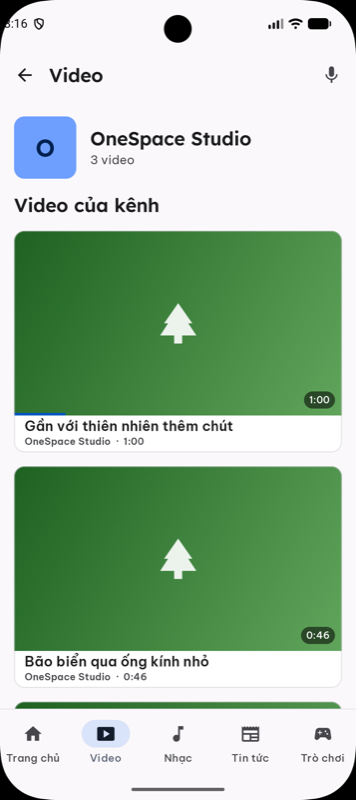
\includegraphics[height=6.1cm]{../figures/app/F-VID-12-01.png}
\end{column}
\end{columns}
\end{frame}

\begin{frame}{Mock Up: Phân hệ Video (1/2)}
\begin{columns}[T]
\begin{column}{0.46\textwidth}
{\small\bfseries\color{BKTemplate} F-VID-13: Playlist video theo chủ đề}\\[2.5mm]
Tính năng thuộc nhóm Fill-ins
\end{column}
\begin{column}{0.50\textwidth}
\centering
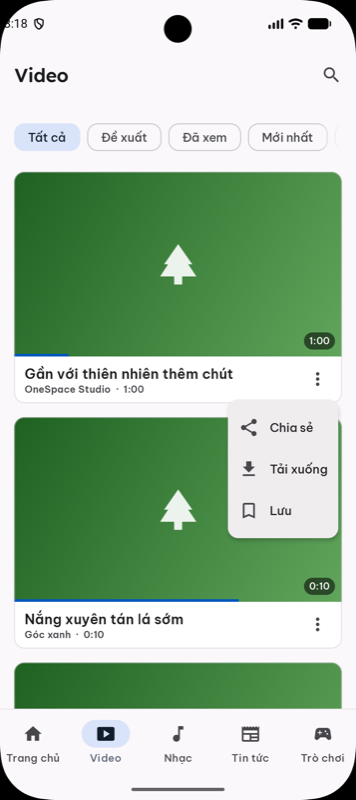
\includegraphics[width=2.75cm]{../figures/app/F-VID-13-01.png}\hspace{0.25cm}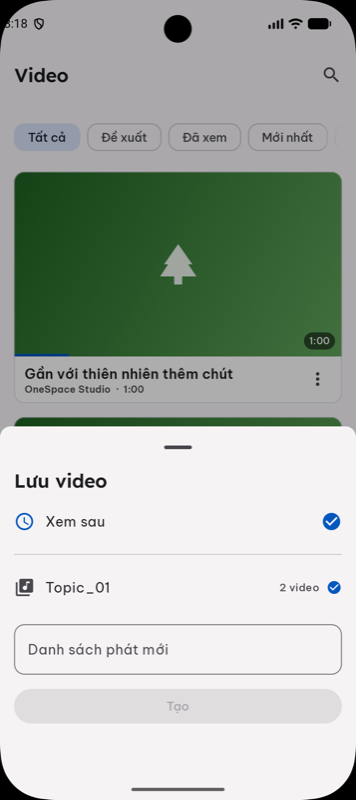
\includegraphics[width=2.75cm]{../figures/app/F-VID-13-02.png}
\end{column}
\end{columns}
\end{frame}

\begin{frame}{Mock Up: Phân hệ Video (2/2)}
\begin{columns}[T]
\begin{column}{0.46\textwidth}
{\small\bfseries\color{BKTemplate} F-VID-13: Playlist video theo chủ đề}\\[2.5mm]
Tính năng thuộc nhóm Fill-ins
\end{column}
\begin{column}{0.50\textwidth}
\centering
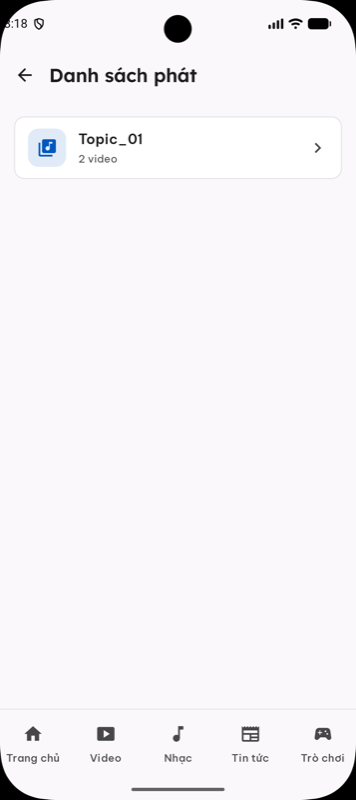
\includegraphics[width=2.75cm]{../figures/app/F-VID-13-03.png}\hspace{0.25cm}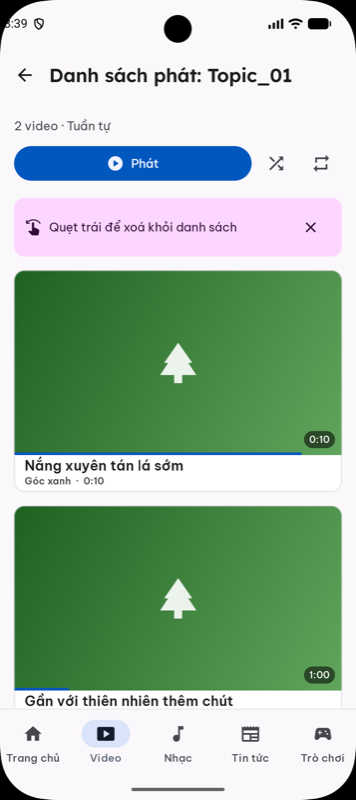
\includegraphics[width=2.75cm]{../figures/app/F-VID-13-04.png}
\end{column}
\end{columns}
\end{frame}

\begin{frame}{Mock Up: Phân hệ Video}
\begin{columns}[T]
\begin{column}{0.46\textwidth}
{\small\bfseries\color{BKTemplate} F-VID-14: Tua nhanh double-tap và đổi tốc độ phát}\\[2.5mm]
Tính năng thuộc nhóm Quick Wins
\end{column}
\begin{column}{0.50\textwidth}
\centering
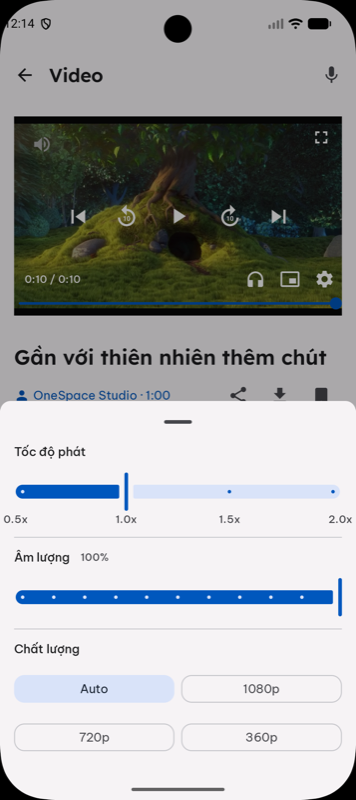
\includegraphics[height=6.1cm]{../figures/app/F-VID-14-01.png}
\end{column}
\end{columns}
\end{frame}

\begin{frame}{Mock Up: Phân hệ Video}
\begin{columns}[T]
\begin{column}{0.46\textwidth}
{\small\bfseries\color{BKTemplate} F-VID-15: Gợi ý ``chơi game liên quan video này'': thẻ game cuối video, câu hỏi soạn sẵn lúc đăng nội dung}\\[2.5mm]
Tính năng thuộc nhóm Quick Wins
\end{column}
\begin{column}{0.50\textwidth}
\centering
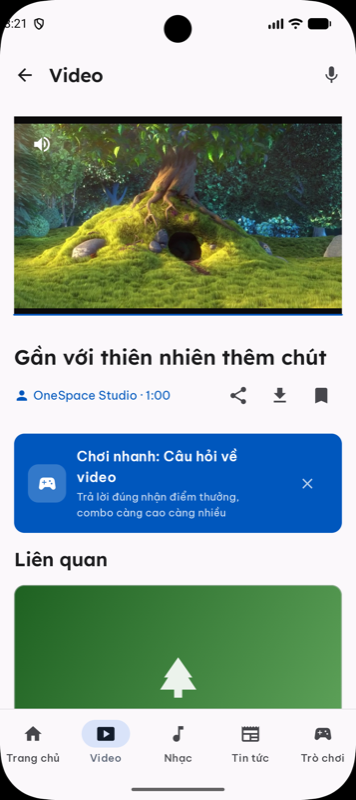
\includegraphics[width=2.75cm]{../figures/app/F-VID-15-01.png}\hspace{0.25cm}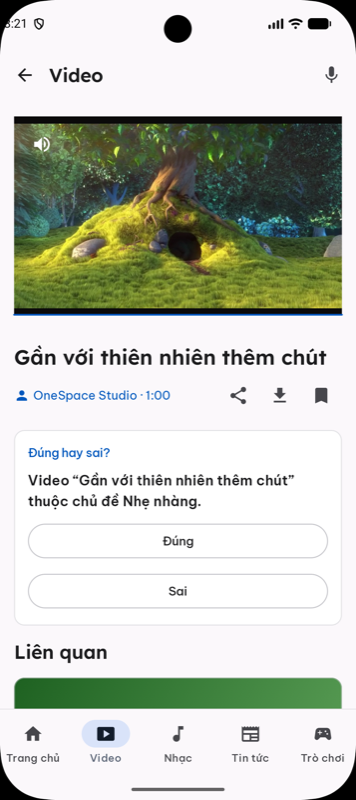
\includegraphics[width=2.75cm]{../figures/app/F-VID-15-02.png}
\end{column}
\end{columns}
\end{frame}

\begin{frame}{Mock Up: Phân hệ Video}
\begin{columns}[T]
\begin{column}{0.46\textwidth}
{\small\bfseries\color{BKTemplate} F-VID-16: Toàn màn hình: nút ẩn system bars, player chiếm cả trang}\\[2.5mm]
Tính năng thuộc nhóm Quick Wins
\end{column}
\begin{column}{0.50\textwidth}
\centering
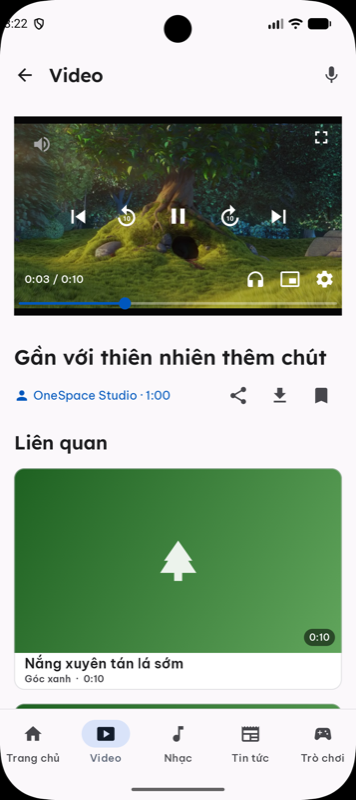
\includegraphics[width=2.75cm]{../figures/app/F-VID-16-01.png}\hspace{0.25cm}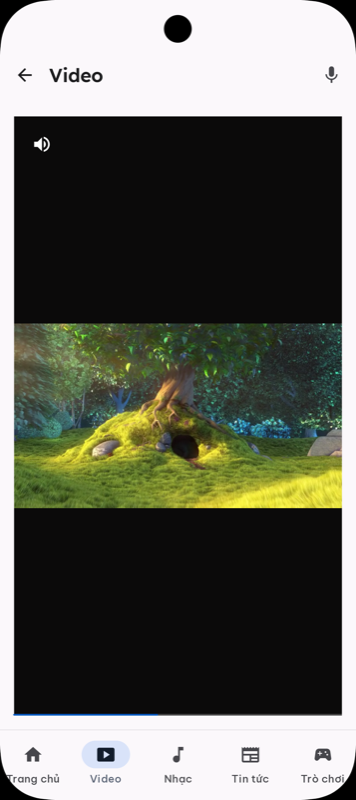
\includegraphics[width=2.75cm]{../figures/app/F-VID-16-02.png}
\end{column}
\end{columns}
\end{frame}

\begin{frame}{Mock Up: Phân hệ Video}
\begin{columns}[T]
\begin{column}{0.46\textwidth}
{\small\bfseries\color{BKTemplate} F-VID-17: Điều khiển âm lượng: nút loa mute/unmute + thanh volume hệ thống}\\[2.5mm]
Tính năng thuộc nhóm Quick Wins
\end{column}
\begin{column}{0.50\textwidth}
\centering
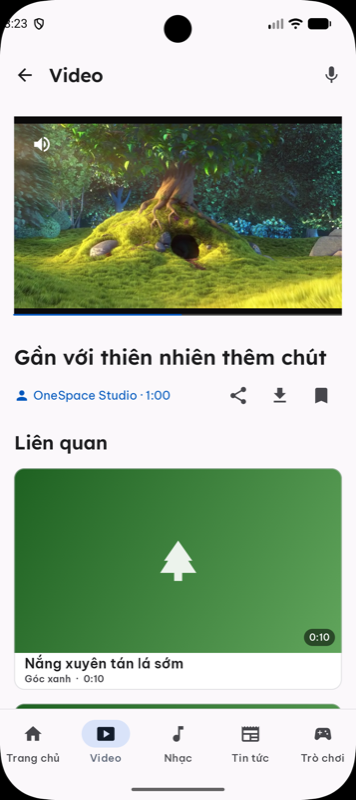
\includegraphics[height=6.1cm]{../figures/app/F-VID-17-01.png}
\end{column}
\end{columns}
\end{frame}

\begin{frame}{Mock Up: Phân hệ Video}
\begin{columns}[T]
\begin{column}{0.46\textwidth}
{\small\bfseries\color{BKTemplate} F-VID-18: Pinch-to-zoom cửa sổ nổi: 2 ngón thu phóng 0.5x--2x}\\[2.5mm]
Tính năng thuộc nhóm Fill-ins
\end{column}
\begin{column}{0.50\textwidth}
\centering
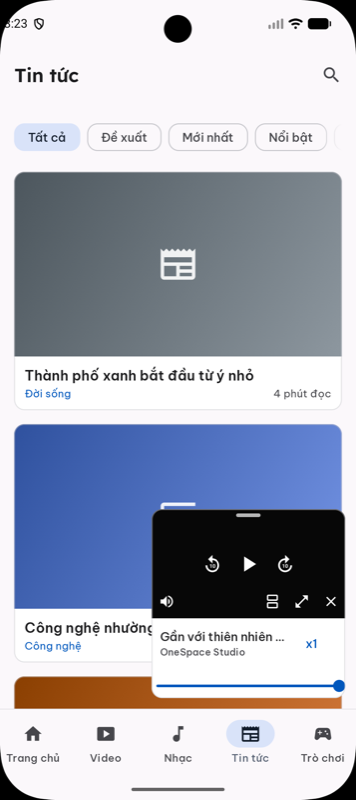
\includegraphics[height=6.1cm]{../figures/app/F-VID-18-01.png}
\end{column}
\end{columns}
\end{frame}

\begin{frame}{Mock Up: Phân hệ Nhạc}
\begin{columns}[T]
\begin{column}{0.46\textwidth}
{\small\bfseries\color{BKTemplate} F-MUS-01: Player nhạc đầy đủ (phát / dừng / chuyển / tua / repeat / shuffle)}\\[2.5mm]
Tính năng thuộc nhóm Major Projects
\end{column}
\begin{column}{0.50\textwidth}
\centering
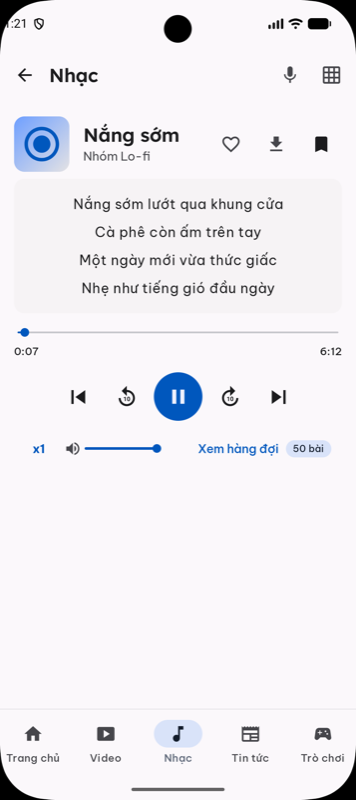
\includegraphics[width=2.75cm]{../figures/app/F-MUS-01-01.png}\hspace{0.25cm}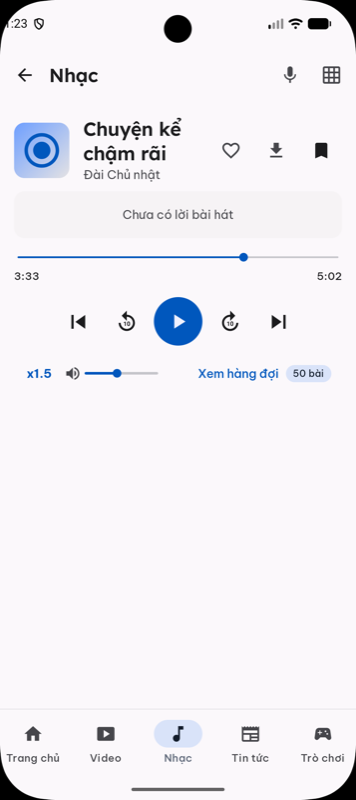
\includegraphics[width=2.75cm]{../figures/app/F-MUS-01-02.png}
\end{column}
\end{columns}
\end{frame}

\begin{frame}{Mock Up: Phân hệ Nhạc}
\begin{columns}[T]
\begin{column}{0.46\textwidth}
{\small\bfseries\color{BKTemplate} F-MUS-02: Mini player dock xuyên suốt mọi màn hình}\\[2.5mm]
Tính năng thuộc nhóm Major Projects
\end{column}
\begin{column}{0.50\textwidth}
\centering
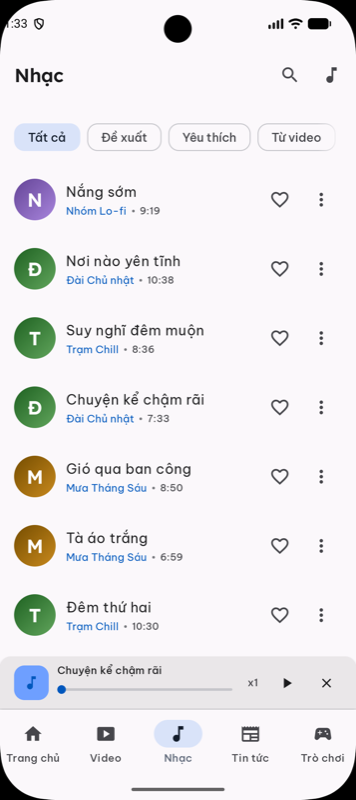
\includegraphics[width=2.75cm]{../figures/app/F-MUS-02-01.png}\hspace{0.25cm}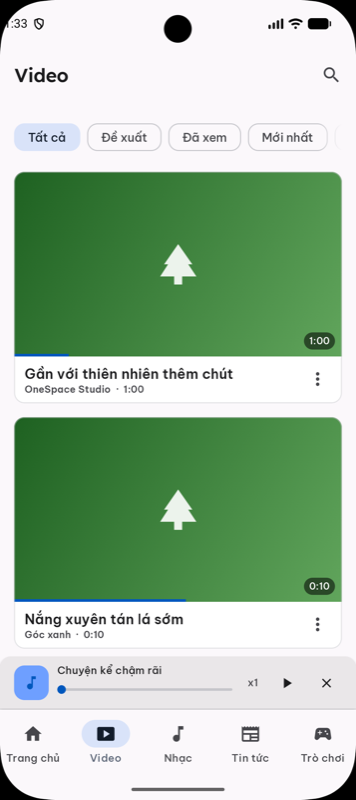
\includegraphics[width=2.75cm]{../figures/app/F-MUS-02-02.png}
\end{column}
\end{columns}
\end{frame}

\begin{frame}{Mock Up: Phân hệ Nhạc}
\begin{columns}[T]
\begin{column}{0.46\textwidth}
{\small\bfseries\color{BKTemplate} F-MUS-03: Phát nhạc nền khi rời ứng dụng hoặc khoá màn hình}\\[2.5mm]
Tính năng thuộc nhóm Major Projects
\end{column}
\begin{column}{0.50\textwidth}
\centering
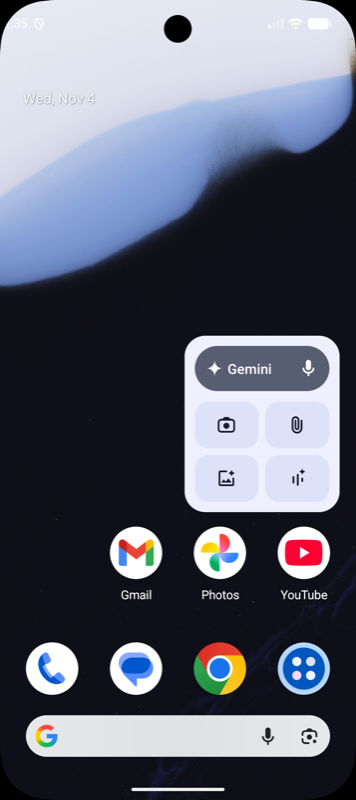
\includegraphics[height=6.1cm]{../figures/app/F-MUS-03-01.png}
\end{column}
\end{columns}
\end{frame}

\begin{frame}{Mock Up: Phân hệ Nhạc}
\begin{columns}[T]
\begin{column}{0.46\textwidth}
{\small\bfseries\color{BKTemplate} F-MUS-04: Tự tạo/sửa/xoá playlist}\\[2.5mm]
Tính năng thuộc nhóm Quick Wins
\end{column}
\begin{column}{0.50\textwidth}
\centering
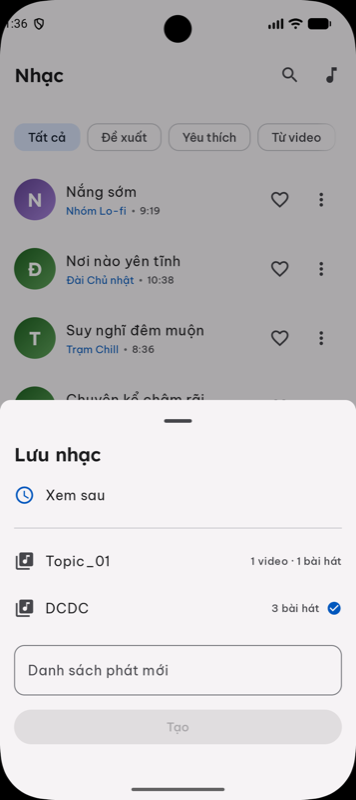
\includegraphics[width=2.75cm]{../figures/app/F-MUS-04-01.png}\hspace{0.25cm}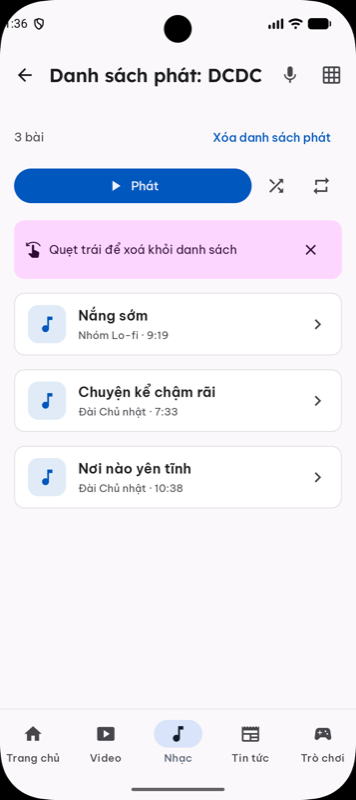
\includegraphics[width=2.75cm]{../figures/app/F-MUS-04-02.png}
\end{column}
\end{columns}
\end{frame}

\begin{frame}{Mock Up: Phân hệ Nhạc}
\begin{columns}[T]
\begin{column}{0.46\textwidth}
{\small\bfseries\color{BKTemplate} F-MUS-05: Hàng phát (queue): thêm tiếp theo, phát cuối, kéo sắp lại}\\[2.5mm]
Tính năng thuộc nhóm Quick Wins
\end{column}
\begin{column}{0.50\textwidth}
\centering
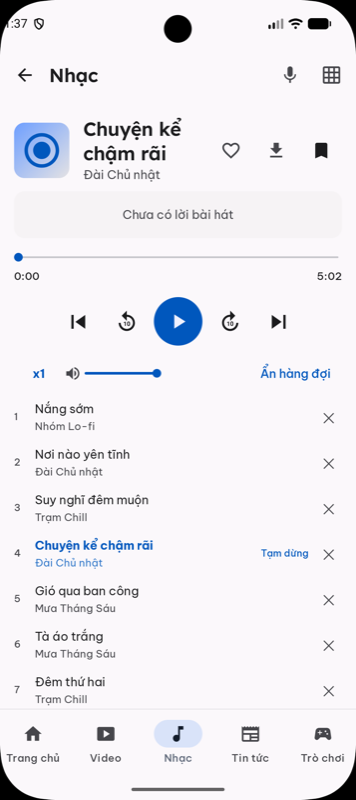
\includegraphics[width=2.75cm]{../figures/app/F-MUS-05-01.png}\hspace{0.25cm}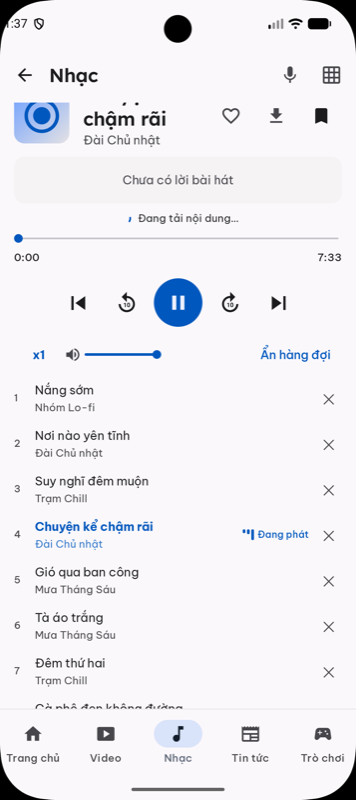
\includegraphics[width=2.75cm]{../figures/app/F-MUS-05-02.png}
\end{column}
\end{columns}
\end{frame}

\begin{frame}{Mock Up: Phân hệ Nhạc}
\begin{columns}[T]
\begin{column}{0.46\textwidth}
{\small\bfseries\color{BKTemplate} F-MUS-06: Tìm kiếm nhạc (bài hát/nghệ sĩ/album)}\\[2.5mm]
Tính năng thuộc nhóm Quick Wins
\end{column}
\begin{column}{0.50\textwidth}
\centering
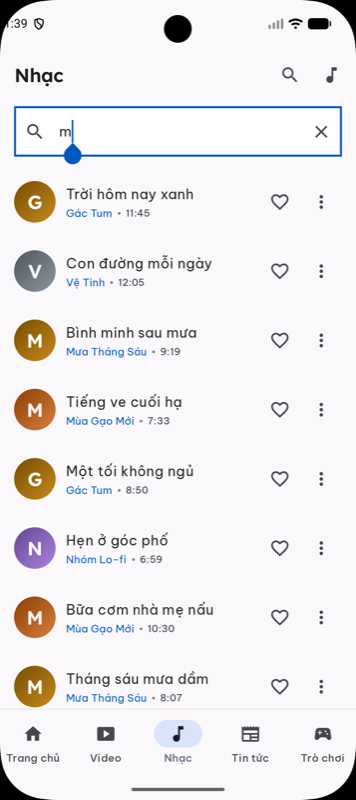
\includegraphics[height=6.1cm]{../figures/app/F-MUS-06-01.png}
\end{column}
\end{columns}
\end{frame}

\begin{frame}{Mock Up: Phân hệ Nhạc}
\begin{columns}[T]
\begin{column}{0.46\textwidth}
{\small\bfseries\color{BKTemplate} F-MUS-07: Kho nhạc cá nhân chứa các tệp trích từ video}\\[2.5mm]
Tính năng thuộc nhóm Major Projects
\end{column}
\begin{column}{0.50\textwidth}
\centering
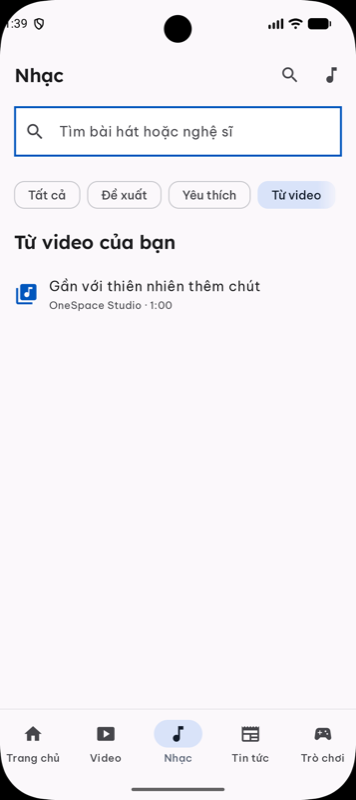
\includegraphics[height=6.1cm]{../figures/app/F-MUS-07-01.png}
\end{column}
\end{columns}
\end{frame}

\begin{frame}{Mock Up: Phân hệ Nhạc}
\begin{columns}[T]
\begin{column}{0.46\textwidth}
{\small\bfseries\color{BKTemplate} F-MUS-08: Gợi ý nhạc theo sở thích}\\[2.5mm]
Tính năng thuộc nhóm Major Projects
\end{column}
\begin{column}{0.50\textwidth}
\centering
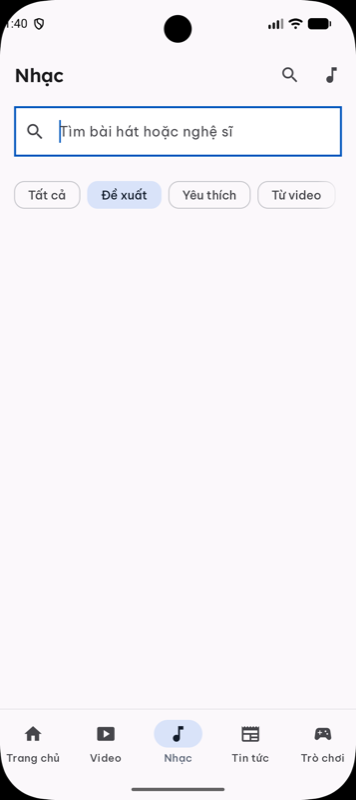
\includegraphics[height=6.1cm]{../figures/app/F-MUS-08-01.png}
\end{column}
\end{columns}
\end{frame}

\begin{frame}{Mock Up: Phân hệ Nhạc}
\begin{columns}[T]
\begin{column}{0.46\textwidth}
{\small\bfseries\color{BKTemplate} F-MUS-09: ``Siêu playlist'' (meta-playlist) trộn nhạc và video}\\[2.5mm]
Tính năng thuộc nhóm Major Projects
\end{column}
\begin{column}{0.50\textwidth}
\centering
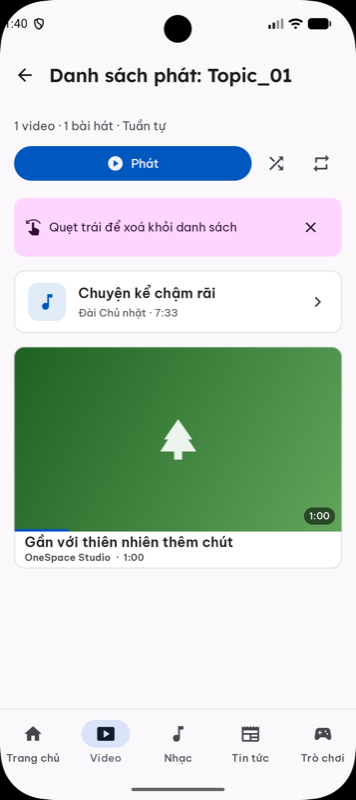
\includegraphics[height=6.1cm]{../figures/app/F-MUS-09-01.png}
\end{column}
\end{columns}
\end{frame}

\begin{frame}{Mock Up: Phân hệ Nhạc}
\begin{columns}[T]
\begin{column}{0.46\textwidth}
{\small\bfseries\color{BKTemplate} F-MUS-10: Xử lý audio focus: duck/pause khi có luồng âm thanh khác}\\[2.5mm]
Tính năng thuộc nhóm Major Projects
\end{column}
\begin{column}{0.50\textwidth}
\centering
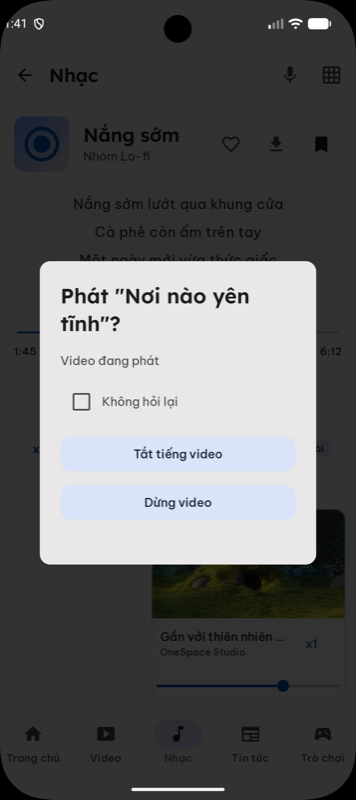
\includegraphics[height=6.1cm]{../figures/app/F-MUS-10-01.png}
\end{column}
\end{columns}
\end{frame}

\begin{frame}{Mock Up: Phân hệ Nhạc}
\begin{columns}[T]
\begin{column}{0.46\textwidth}
{\small\bfseries\color{BKTemplate} F-MUS-12: Tải bài hát offline}\\[2.5mm]
Tính năng thuộc nhóm Thankless
\end{column}
\begin{column}{0.50\textwidth}
\centering
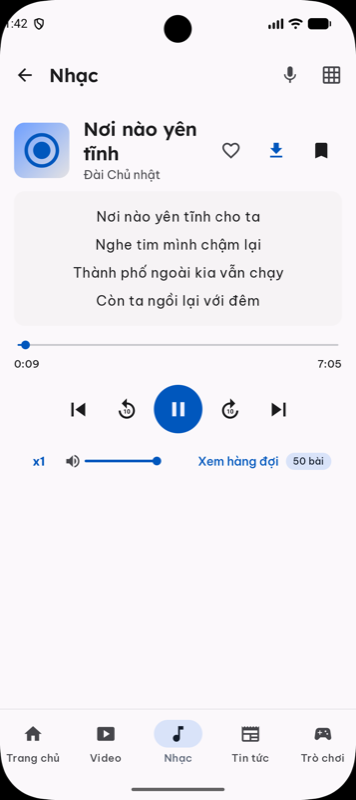
\includegraphics[width=2.75cm]{../figures/app/F-MUS-12-01.png}\hspace{0.25cm}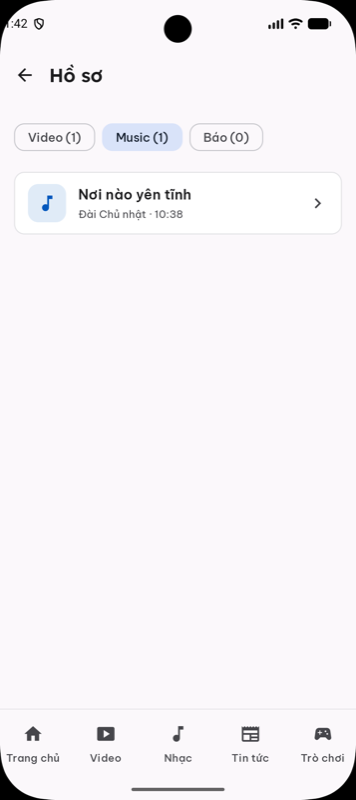
\includegraphics[width=2.75cm]{../figures/app/F-MUS-12-02.png}
\end{column}
\end{columns}
\end{frame}

\begin{frame}{Mock Up: Phân hệ Nhạc}
\begin{columns}[T]
\begin{column}{0.46\textwidth}
{\small\bfseries\color{BKTemplate} F-MUS-13: Tốc độ phát nhạc: x1/x1.5/x2/x0.5 trên dock và Home card}\\[2.5mm]
Tính năng thuộc nhóm Quick Wins
\end{column}
\begin{column}{0.50\textwidth}
\centering
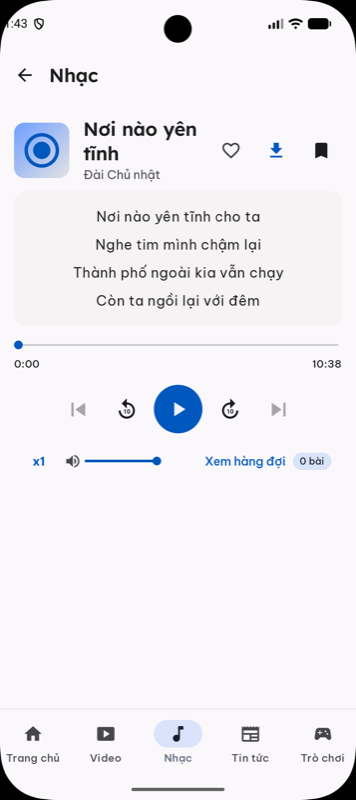
\includegraphics[width=2.75cm]{../figures/app/F-MUS-13-01.png}\hspace{0.25cm}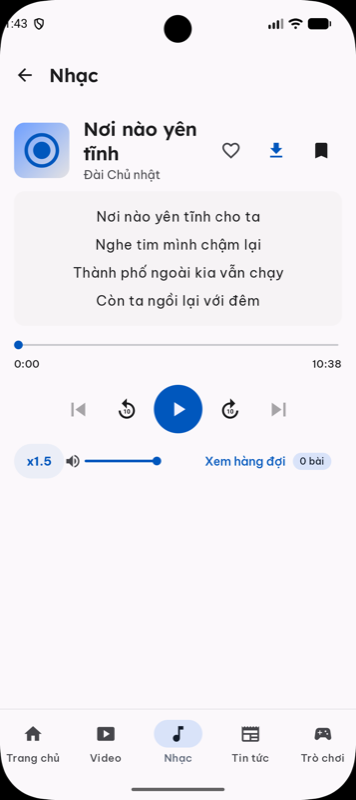
\includegraphics[width=2.75cm]{../figures/app/F-MUS-13-02.png}
\end{column}
\end{columns}
\end{frame}

\begin{frame}{Mock Up: Phân hệ Nhạc}
\begin{columns}[T]
\begin{column}{0.46\textwidth}
{\small\bfseries\color{BKTemplate} F-MUS-14: Lời bài hát: panel scroll trên Now Playing}\\[2.5mm]
Tính năng thuộc nhóm Fill-ins
\end{column}
\begin{column}{0.50\textwidth}
\centering
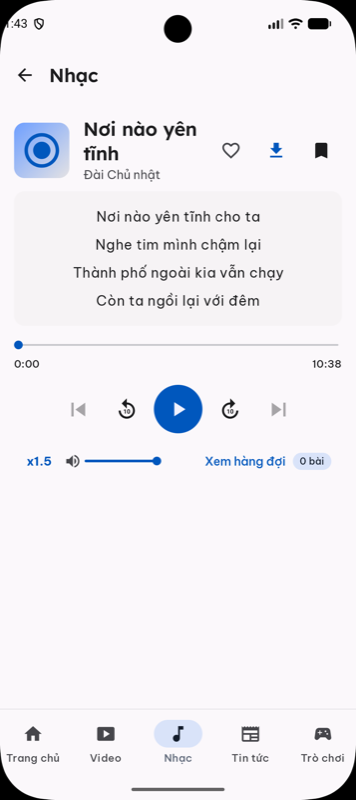
\includegraphics[height=6.1cm]{../figures/app/F-MUS-14-01.png}
\end{column}
\end{columns}
\end{frame}

\begin{frame}{Mock Up: Phân hệ Tin tức}
\begin{columns}[T]
\begin{column}{0.46\textwidth}
{\small\bfseries\color{BKTemplate} F-NEWS-01: Feed tin theo chuyên mục và sở thích}\\[2.5mm]
Tính năng thuộc nhóm Major Projects
\end{column}
\begin{column}{0.50\textwidth}
\centering
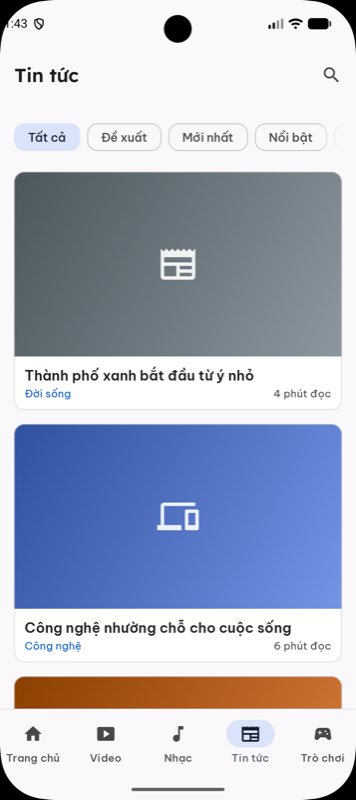
\includegraphics[width=2.75cm]{../figures/app/F-NEWS-01-01.png}\hspace{0.25cm}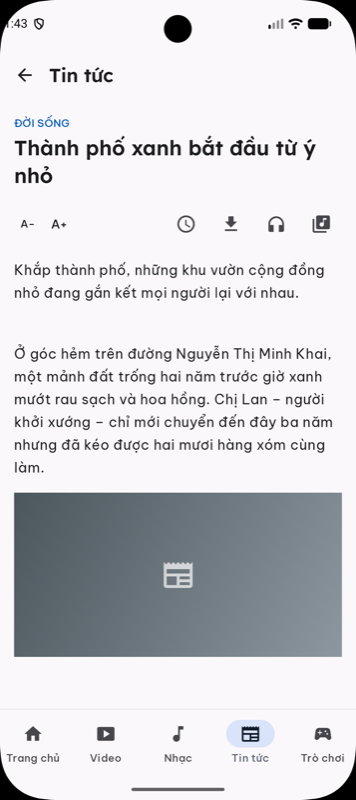
\includegraphics[width=2.75cm]{../figures/app/F-NEWS-01-02.png}
\end{column}
\end{columns}
\end{frame}

\begin{frame}{Mock Up: Phân hệ Tin tức}
\begin{columns}[T]
\begin{column}{0.46\textwidth}
{\small\bfseries\color{BKTemplate} F-NEWS-02: Trình đọc sạch, đổi cỡ chữ}\\[2.5mm]
Tính năng thuộc nhóm Quick Wins
\end{column}
\begin{column}{0.50\textwidth}
\centering
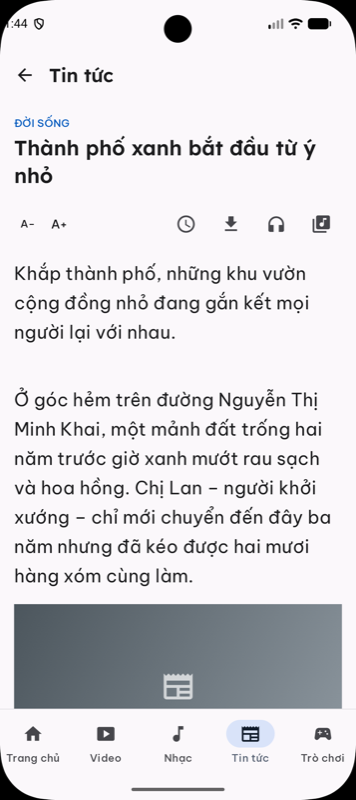
\includegraphics[height=6.1cm]{../figures/app/F-NEWS-02-01.png}
\end{column}
\end{columns}
\end{frame}

\begin{frame}{Mock Up: Phân hệ Tin tức}
\begin{columns}[T]
\begin{column}{0.46\textwidth}
{\small\bfseries\color{BKTemplate} F-NEWS-03: Lưu bài đọc sau}\\[2.5mm]
Tính năng thuộc nhóm Quick Wins
\end{column}
\begin{column}{0.50\textwidth}
\centering
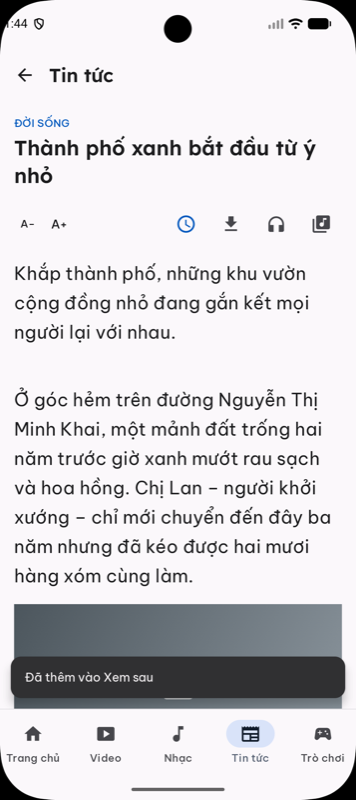
\includegraphics[height=6.1cm]{../figures/app/F-NEWS-03-01.png}
\end{column}
\end{columns}
\end{frame}

\begin{frame}{Mock Up: Phân hệ Tin tức}
\begin{columns}[T]
\begin{column}{0.46\textwidth}
{\small\bfseries\color{BKTemplate} F-NEWS-04: Tìm kiếm bài báo}\\[2.5mm]
Tính năng thuộc nhóm Fill-ins
\end{column}
\begin{column}{0.50\textwidth}
\centering
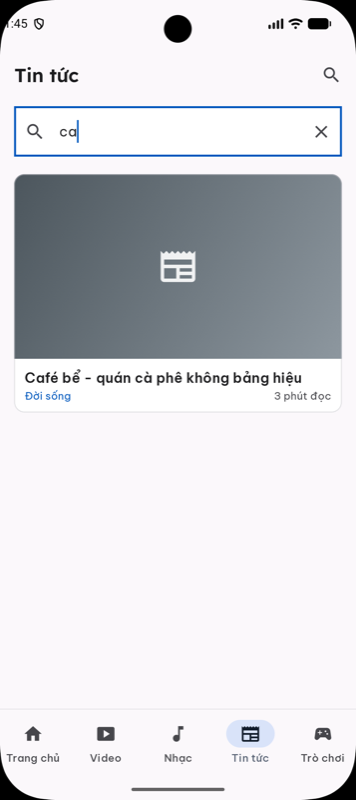
\includegraphics[height=6.1cm]{../figures/app/F-NEWS-04-01.png}
\end{column}
\end{columns}
\end{frame}

\begin{frame}{Mock Up: Phân hệ Tin tức}
\begin{columns}[T]
\begin{column}{0.46\textwidth}
{\small\bfseries\color{BKTemplate} F-NEWS-05: Chuyển bài báo thành audio (TTS)~--~``nghe tin''}\\[2.5mm]
Tính năng thuộc nhóm Major Projects
\end{column}
\begin{column}{0.50\textwidth}
\centering
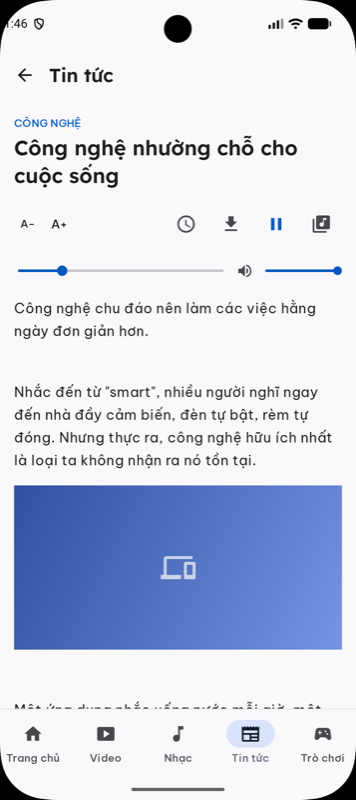
\includegraphics[width=2.75cm]{../figures/app/F-NEWS-05-01.png}\hspace{0.25cm}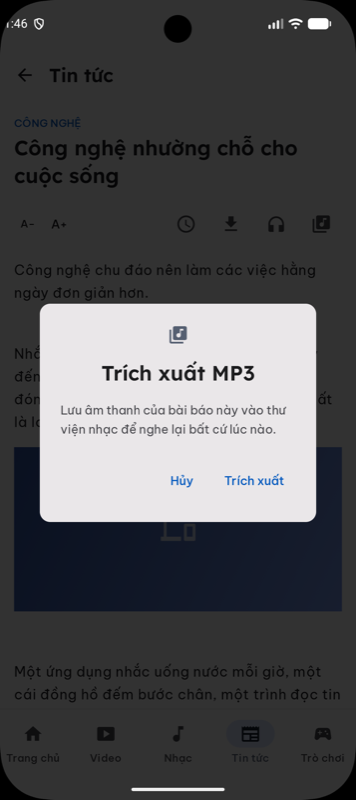
\includegraphics[width=2.75cm]{../figures/app/F-NEWS-05-02.png}
\end{column}
\end{columns}
\end{frame}

\begin{frame}{Mock Up: Phân hệ Tin tức}
\begin{columns}[T]
\begin{column}{0.46\textwidth}
{\small\bfseries\color{BKTemplate} F-NEWS-06: Sắp xếp mới nhất / phổ biến}\\[2.5mm]
Tính năng thuộc nhóm Quick Wins
\end{column}
\begin{column}{0.50\textwidth}
\centering
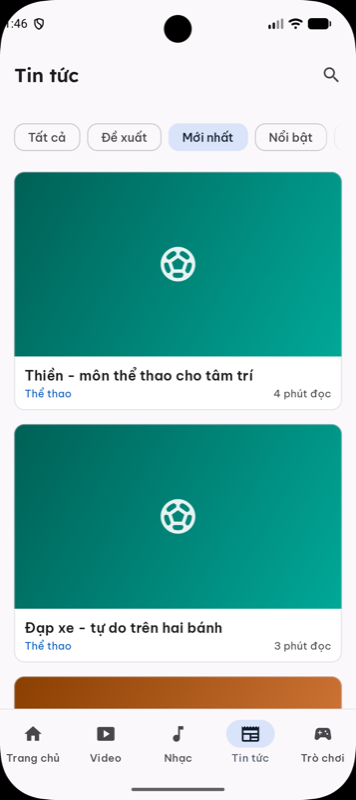
\includegraphics[height=6.1cm]{../figures/app/F-NEWS-06-01.png}
\end{column}
\end{columns}
\end{frame}

\begin{frame}{Mock Up: Phân hệ Tin tức}
\begin{columns}[T]
\begin{column}{0.46\textwidth}
{\small\bfseries\color{BKTemplate} F-NEWS-07: Nghe nhạc khi đọc tin (dock vẫn phát)}\\[2.5mm]
Tính năng thuộc nhóm Quick Wins
\end{column}
\begin{column}{0.50\textwidth}
\centering
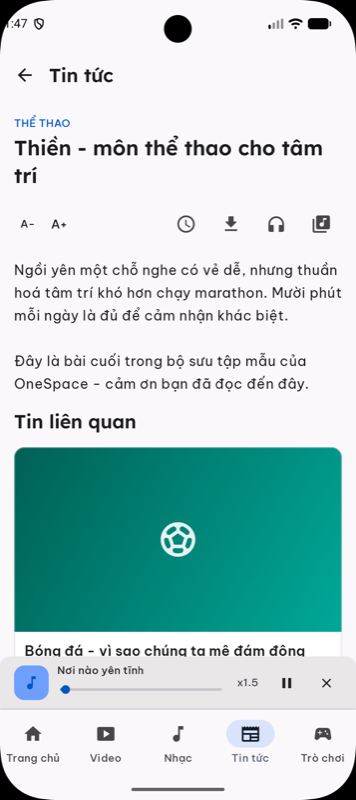
\includegraphics[height=6.1cm]{../figures/app/F-NEWS-07-01.png}
\end{column}
\end{columns}
\end{frame}

\begin{frame}{Mock Up: Phân hệ Tin tức}
\begin{columns}[T]
\begin{column}{0.46\textwidth}
{\small\bfseries\color{BKTemplate} F-NEWS-08: Quiz sinh ra từ bài báo đang đọc}\\[2.5mm]
Tính năng thuộc nhóm Major Projects
\end{column}
\begin{column}{0.50\textwidth}
\centering
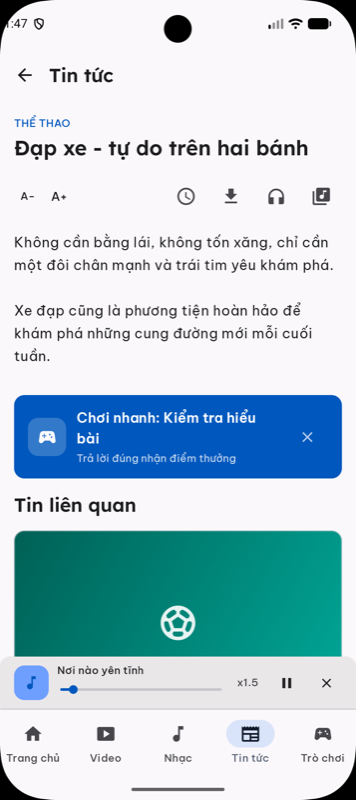
\includegraphics[width=2.75cm]{../figures/app/F-NEWS-08-01.png}\hspace{0.25cm}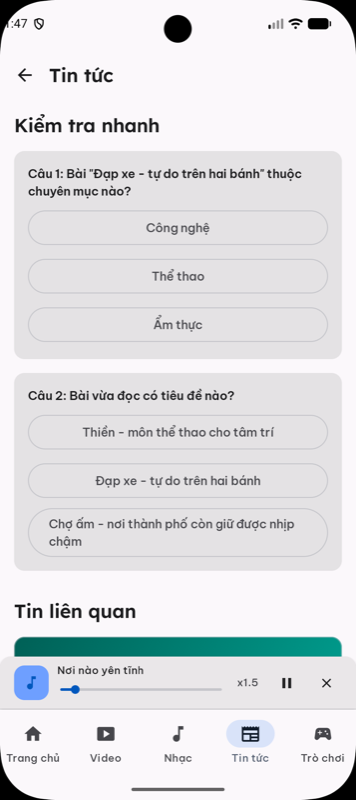
\includegraphics[width=2.75cm]{../figures/app/F-NEWS-08-02.png}
\end{column}
\end{columns}
\end{frame}

\begin{frame}{Mock Up: Phân hệ Tin tức}
\begin{columns}[T]
\begin{column}{0.46\textwidth}
{\small\bfseries\color{BKTemplate} F-NEWS-09: Gợi ý bài liên quan}\\[2.5mm]
Tính năng thuộc nhóm Fill-ins
\end{column}
\begin{column}{0.50\textwidth}
\centering
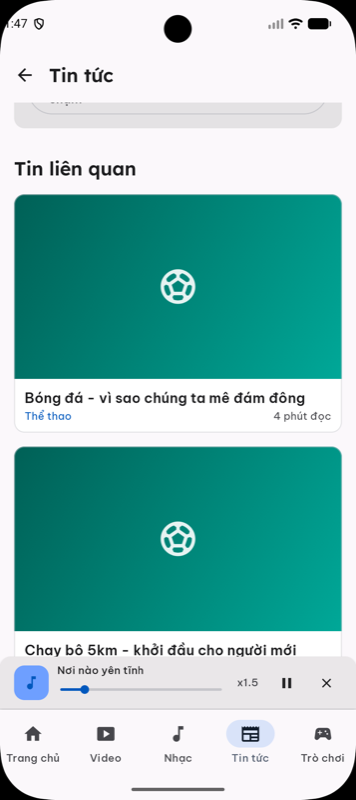
\includegraphics[height=6.1cm]{../figures/app/F-NEWS-09-01.png}
\end{column}
\end{columns}
\end{frame}

\begin{frame}{Mock Up: Phân hệ Tin tức}
\begin{columns}[T]
\begin{column}{0.46\textwidth}
{\small\bfseries\color{BKTemplate} F-NEWS-10: Bài đang đọc thu nhỏ thành thẻ nổi khi rời tab News}\\[2.5mm]
Tính năng thuộc nhóm Major Projects
\end{column}
\begin{column}{0.50\textwidth}
\centering
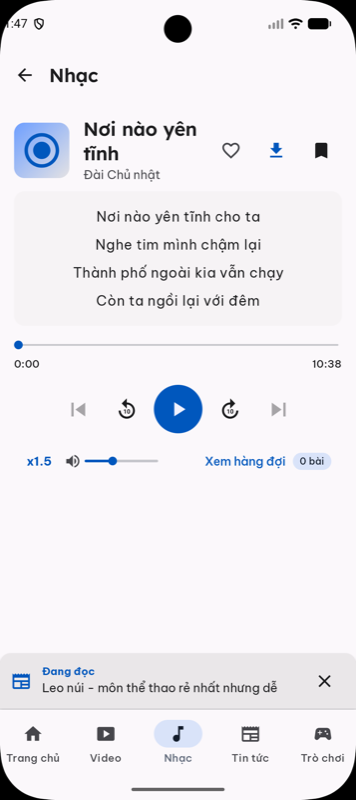
\includegraphics[width=2.75cm]{../figures/app/F-NEWS-10-01.png}\hspace{0.25cm}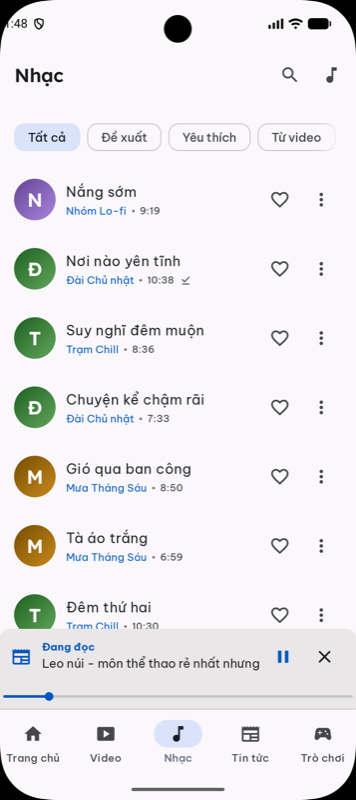
\includegraphics[width=2.75cm]{../figures/app/F-NEWS-10-02.png}
\end{column}
\end{columns}
\end{frame}

\begin{frame}{Mock Up: Phân hệ Trò chơi}
\begin{columns}[T]
\begin{column}{0.46\textwidth}
{\small\bfseries\color{BKTemplate} F-GAME-01: Hub minigame: danh sách, trạng thái mở khoá, phần thưởng}\\[2.5mm]
Tính năng thuộc nhóm Quick Wins
\end{column}
\begin{column}{0.50\textwidth}
\centering
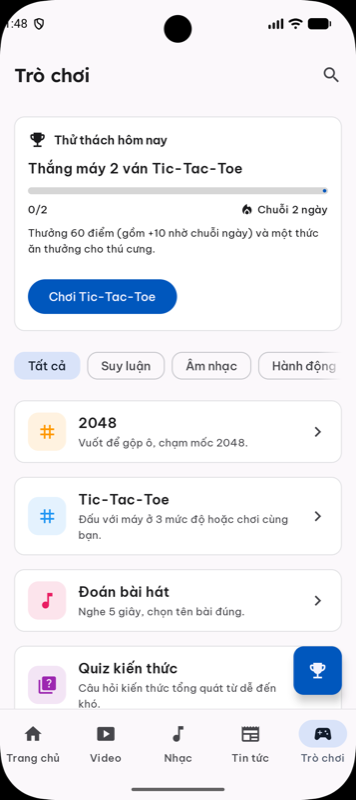
\includegraphics[height=6.1cm]{../figures/app/F-GAME-01-01.png}
\end{column}
\end{columns}
\end{frame}

\begin{frame}{Mock Up: Phân hệ Trò chơi}
\begin{columns}[T]
\begin{column}{0.46\textwidth}
{\small\bfseries\color{BKTemplate} F-GAME-02: Game đoán bài hát}\\[2.5mm]
Tính năng thuộc nhóm Major Projects
\end{column}
\begin{column}{0.50\textwidth}
\centering
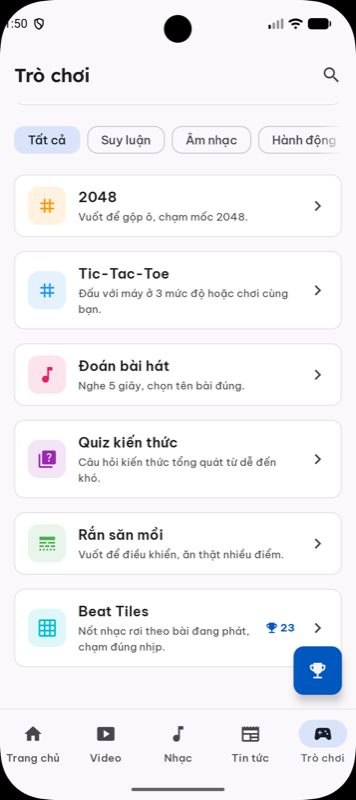
\includegraphics[width=2.32cm]{../figures/app/F-GAME-02-01.png}\hspace{0.2cm}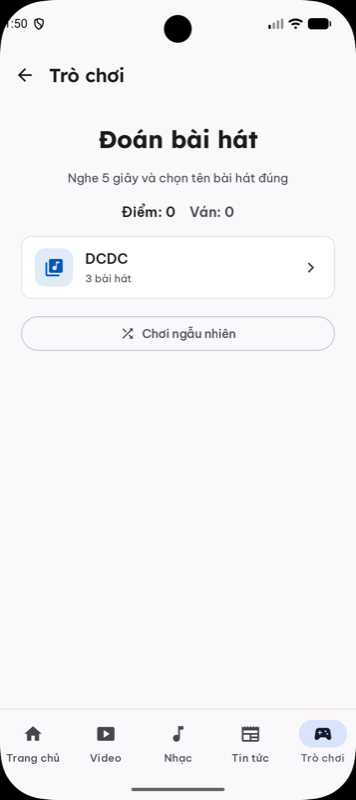
\includegraphics[width=2.32cm]{../figures/app/F-GAME-02-02.png}\hspace{0.2cm}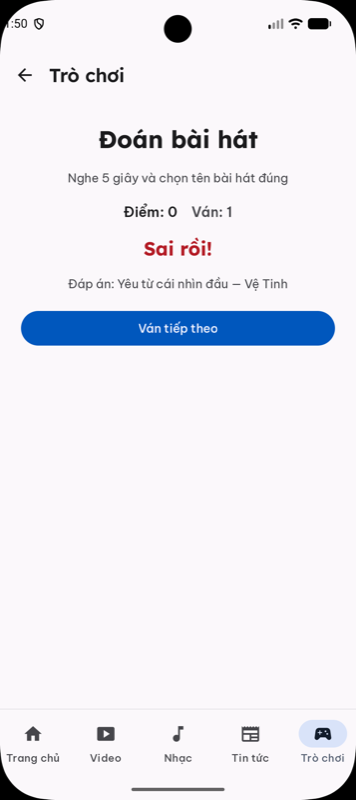
\includegraphics[width=2.32cm]{../figures/app/F-GAME-02-03.png}
\end{column}
\end{columns}
\end{frame}

\begin{frame}{Mock Up: Phân hệ Trò chơi}
\begin{columns}[T]
\begin{column}{0.46\textwidth}
{\small\bfseries\color{BKTemplate} F-GAME-03: Quiz tin tức}\\[2.5mm]
Tính năng thuộc nhóm Major Projects
\end{column}
\begin{column}{0.50\textwidth}
\centering
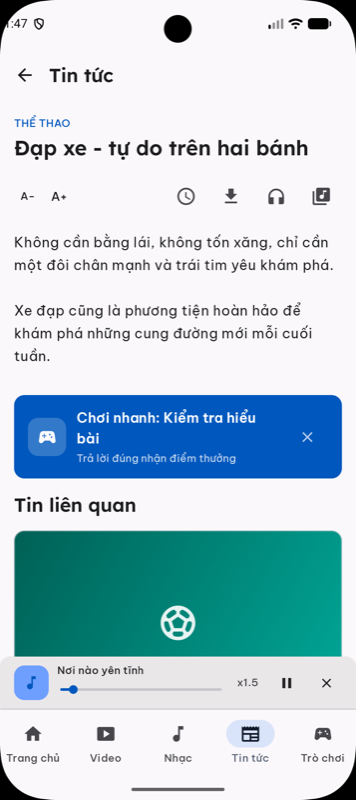
\includegraphics[width=2.75cm]{../figures/app/F-GAME-03-01.png}\hspace{0.25cm}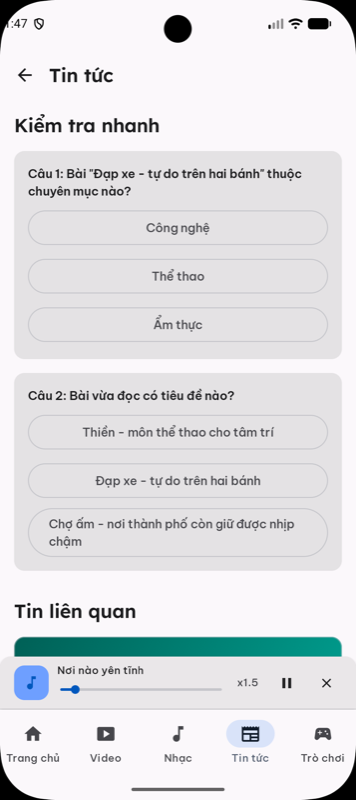
\includegraphics[width=2.75cm]{../figures/app/F-GAME-03-02.png}
\end{column}
\end{columns}
\end{frame}

\begin{frame}{Mock Up: Phân hệ Trò chơi}
\begin{columns}[T]
\begin{column}{0.46\textwidth}
{\small\bfseries\color{BKTemplate} F-GAME-04: Quiz kiến thức (kiểu Ai là triệu phú)}\\[2.5mm]
Tính năng thuộc nhóm Fill-ins
\end{column}
\begin{column}{0.50\textwidth}
\centering
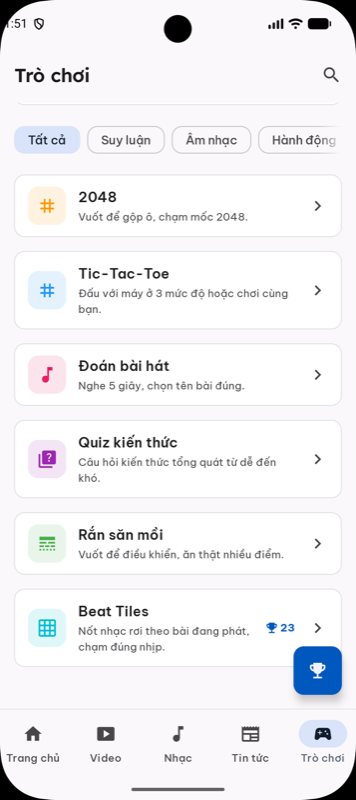
\includegraphics[width=2.32cm]{../figures/app/F-GAME-04-01.png}\hspace{0.2cm}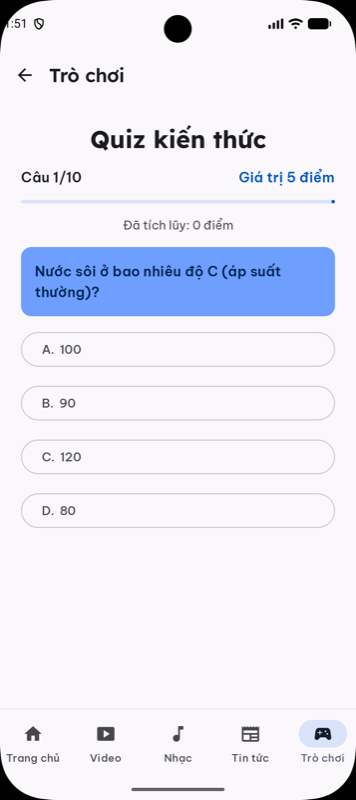
\includegraphics[width=2.32cm]{../figures/app/F-GAME-04-02.png}\hspace{0.2cm}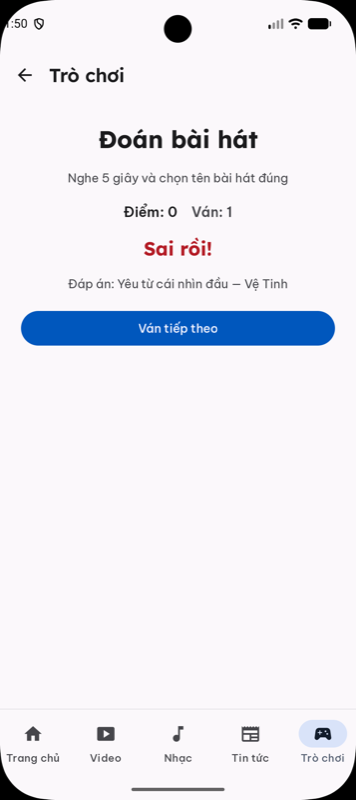
\includegraphics[width=2.32cm]{../figures/app/F-GAME-04-03.png}
\end{column}
\end{columns}
\end{frame}

\begin{frame}{Mock Up: Phân hệ Trò chơi}
\begin{columns}[T]
\begin{column}{0.46\textwidth}
{\small\bfseries\color{BKTemplate} F-GAME-05: Snake -- rắn săn mồi}\\[2.5mm]
Tính năng thuộc nhóm Fill-ins
\end{column}
\begin{column}{0.50\textwidth}
\centering
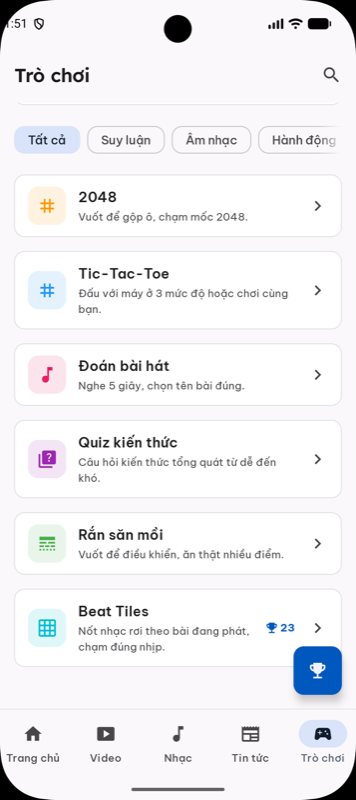
\includegraphics[width=2.32cm]{../figures/app/F-GAME-05-01.png}\hspace{0.2cm}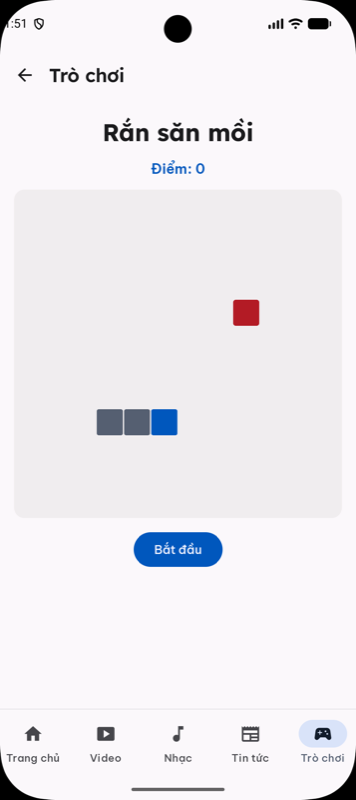
\includegraphics[width=2.32cm]{../figures/app/F-GAME-05-02.png}\hspace{0.2cm}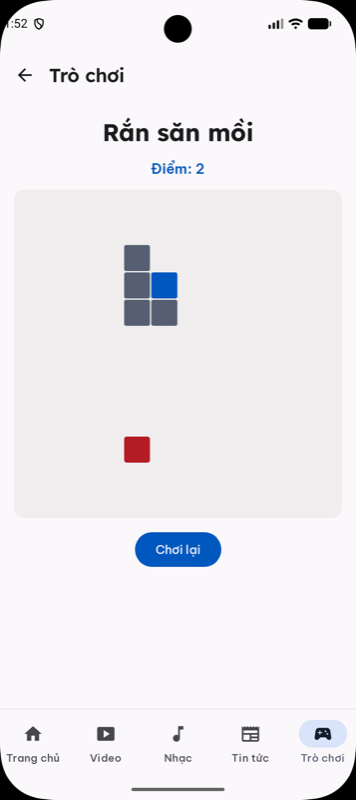
\includegraphics[width=2.32cm]{../figures/app/F-GAME-05-03.png}
\end{column}
\end{columns}
\end{frame}

\begin{frame}{Mock Up: Phân hệ Trò chơi (1/2)}
\begin{columns}[T]
\begin{column}{0.46\textwidth}
{\small\bfseries\color{BKTemplate} F-GAME-06: ``Beat tiles'' -- nốt nhạc rơi theo bài đang phát (kiểu piano tiles)}\\[2.5mm]
Tính năng thuộc nhóm Quick Wins
\end{column}
\begin{column}{0.50\textwidth}
\centering
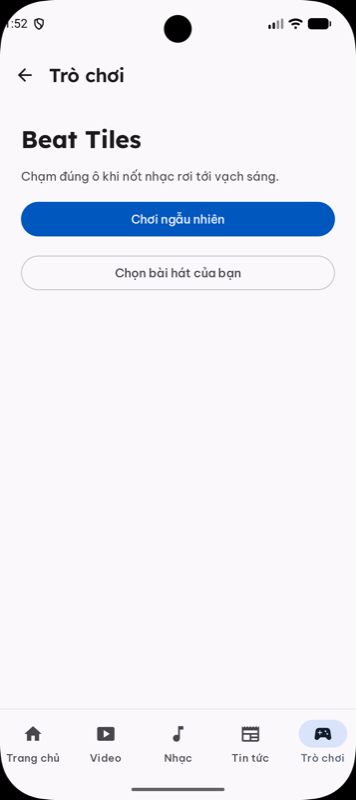
\includegraphics[width=2.75cm]{../figures/app/F-GAME-06-01.png}\hspace{0.25cm}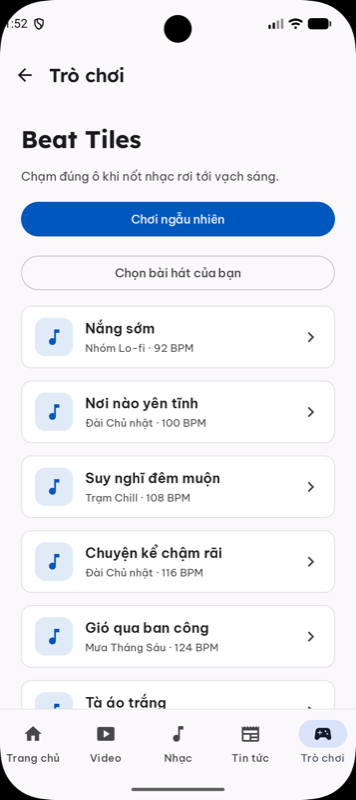
\includegraphics[width=2.75cm]{../figures/app/F-GAME-06-02.png}
\end{column}
\end{columns}
\end{frame}

\begin{frame}{Mock Up: Phân hệ Trò chơi (2/2)}
\begin{columns}[T]
\begin{column}{0.46\textwidth}
{\small\bfseries\color{BKTemplate} F-GAME-06: ``Beat tiles'' -- nốt nhạc rơi theo bài đang phát (kiểu piano tiles)}\\[2.5mm]
Tính năng thuộc nhóm Quick Wins
\end{column}
\begin{column}{0.50\textwidth}
\centering
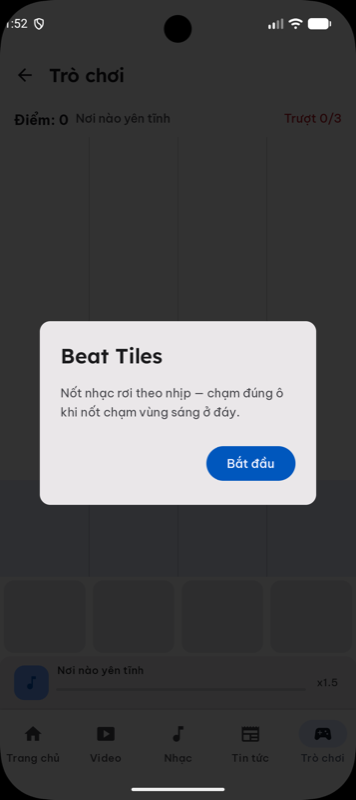
\includegraphics[width=2.75cm]{../figures/app/F-GAME-06-03.png}\hspace{0.25cm}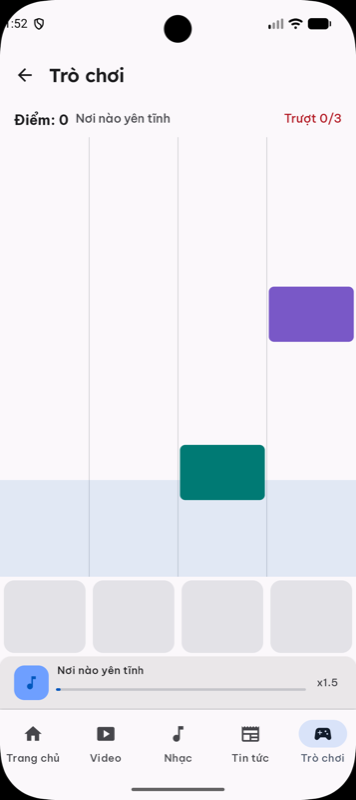
\includegraphics[width=2.75cm]{../figures/app/F-GAME-06-04.png}
\end{column}
\end{columns}
\end{frame}

\begin{frame}{Mock Up: Phân hệ Trò chơi}
\begin{columns}[T]
\begin{column}{0.46\textwidth}
{\small\bfseries\color{BKTemplate} F-GAME-07: Bảng xếp hạng tuần/tháng}\\[2.5mm]
Tính năng thuộc nhóm Major Projects
\end{column}
\begin{column}{0.50\textwidth}
\centering
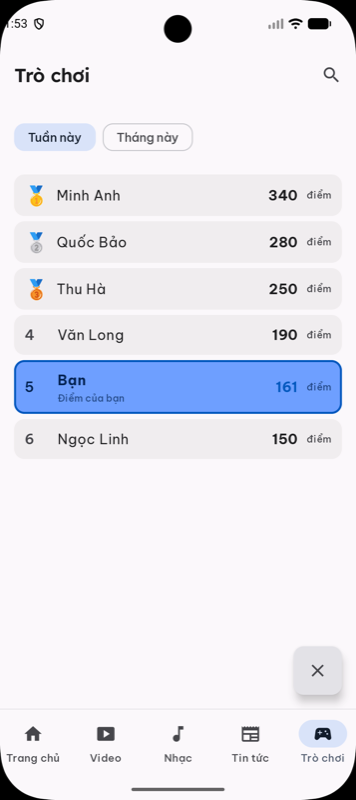
\includegraphics[width=2.75cm]{../figures/app/F-GAME-07-01.png}\hspace{0.25cm}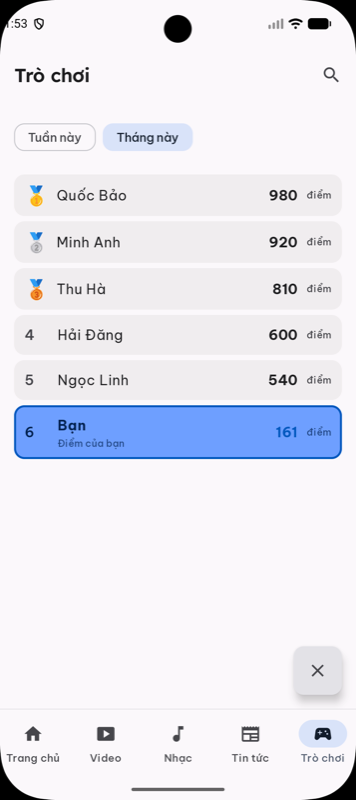
\includegraphics[width=2.75cm]{../figures/app/F-GAME-07-02.png}
\end{column}
\end{columns}
\end{frame}

\begin{frame}{Mock Up: Phân hệ Trò chơi}
\begin{columns}[T]
\begin{column}{0.46\textwidth}
{\small\bfseries\color{BKTemplate} F-GAME-08: Chơi game ở nửa dưới màn hình, video chạy phía trên}\\[2.5mm]
Tính năng thuộc nhóm Major Projects
\end{column}
\begin{column}{0.50\textwidth}
\centering
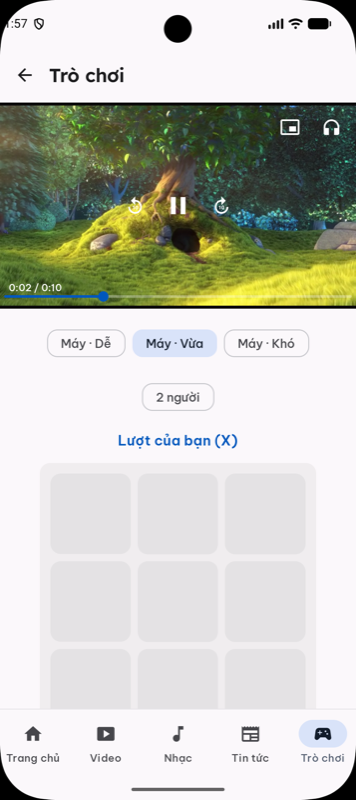
\includegraphics[height=6.1cm]{../figures/app/F-GAME-08-01.png}
\end{column}
\end{columns}
\end{frame}

\begin{frame}{Mock Up: Phân hệ Trò chơi}
\begin{columns}[T]
\begin{column}{0.46\textwidth}
{\small\bfseries\color{BKTemplate} F-GAME-09: Phần thưởng khi thắng minigame (điểm)}\\[2.5mm]
Tính năng thuộc nhóm Quick Wins
\end{column}
\begin{column}{0.50\textwidth}
\centering
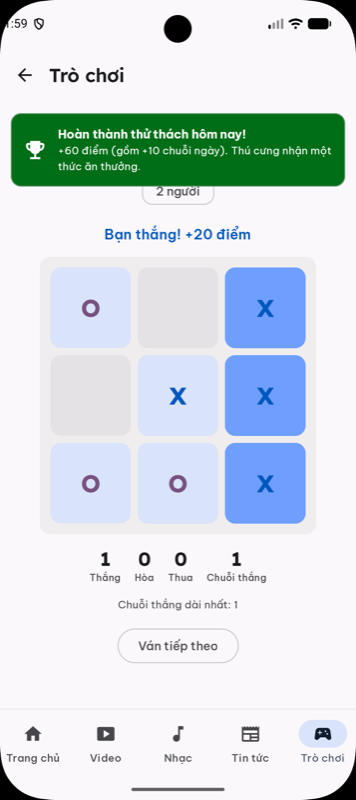
\includegraphics[height=6.1cm]{../figures/app/F-GAME-09-01.png}
\end{column}
\end{columns}
\end{frame}

\begin{frame}{Mock Up: Phân hệ Trò chơi}
\begin{columns}[T]
\begin{column}{0.46\textwidth}
{\small\bfseries\color{BKTemplate} F-GAME-10: 2048 (ghép số)}\\[2.5mm]
Tính năng thuộc nhóm Fill-ins
\end{column}
\begin{column}{0.50\textwidth}
\centering
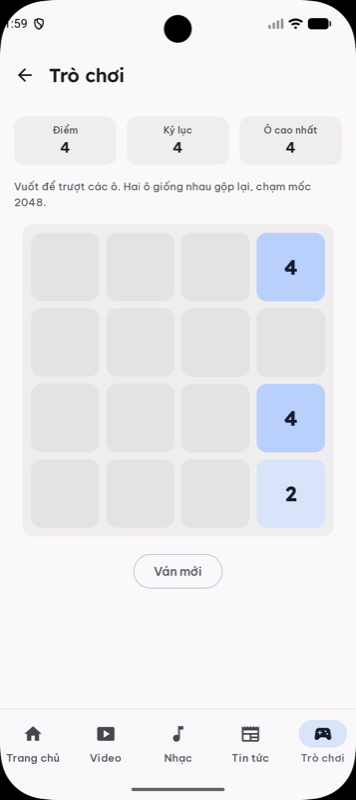
\includegraphics[height=6.1cm]{../figures/app/F-GAME-10-01.png}
\end{column}
\end{columns}
\end{frame}

\begin{frame}{Mock Up: Phân hệ Trò chơi}
\begin{columns}[T]
\begin{column}{0.46\textwidth}
{\small\bfseries\color{BKTemplate} F-GAME-11: Tic-Tac-Toe (caro 3$\times$3)}\\[2.5mm]
Tính năng thuộc nhóm Fill-ins
\end{column}
\begin{column}{0.50\textwidth}
\centering
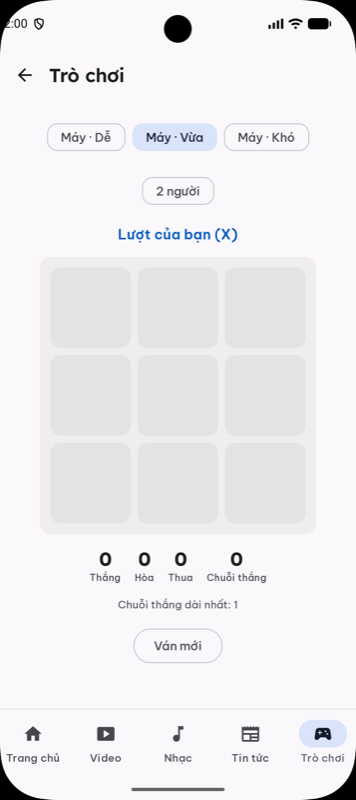
\includegraphics[width=2.75cm]{../figures/app/F-GAME-11-01.png}\hspace{0.25cm}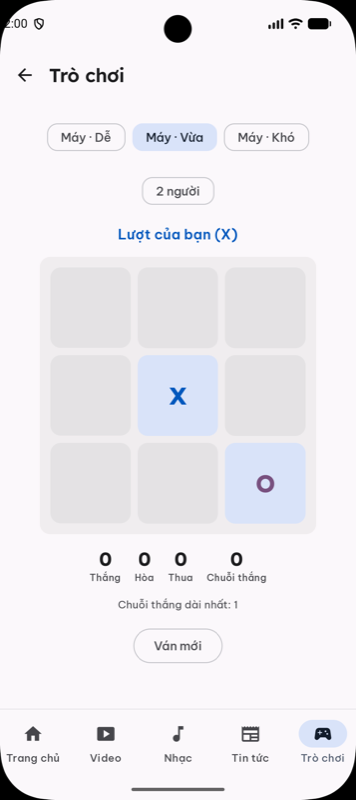
\includegraphics[width=2.75cm]{../figures/app/F-GAME-11-02.png}
\end{column}
\end{columns}
\end{frame}

\begin{frame}{Mock Up: Phân hệ Trò chơi}
\begin{columns}[T]
\begin{column}{0.46\textwidth}
{\small\bfseries\color{BKTemplate} F-GAME-12: Thử thách hằng ngày: xoay vòng 6 game, thưởng 50+5$\times$streak + thức ăn pet}\\[2.5mm]
Tính năng thuộc nhóm Quick Wins
\end{column}
\begin{column}{0.50\textwidth}
\centering
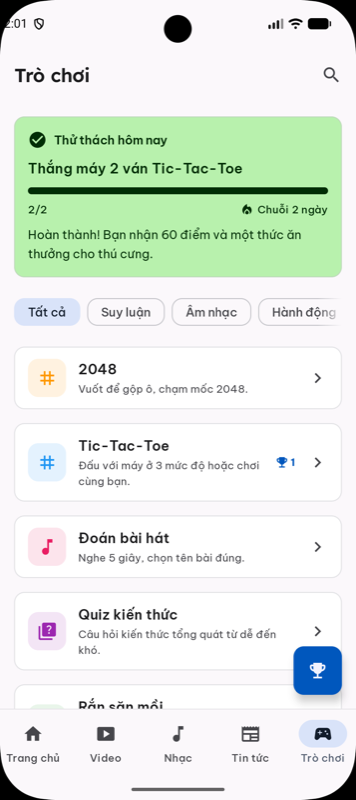
\includegraphics[height=6.1cm]{../figures/app/F-GAME-12-01.png}
\end{column}
\end{columns}
\end{frame}

\begin{frame}{Mock Up: Phân hệ Trò chơi}
\begin{columns}[T]
\begin{column}{0.46\textwidth}
{\small\bfseries\color{BKTemplate} F-GAME-13: Âm thanh và hiệu ứng game: âm phản hồi thao tác, tự giảm khi có nhạc/video}\\[2.5mm]
Tính năng thuộc nhóm Quick Wins
\end{column}
\begin{column}{0.50\textwidth}
\centering
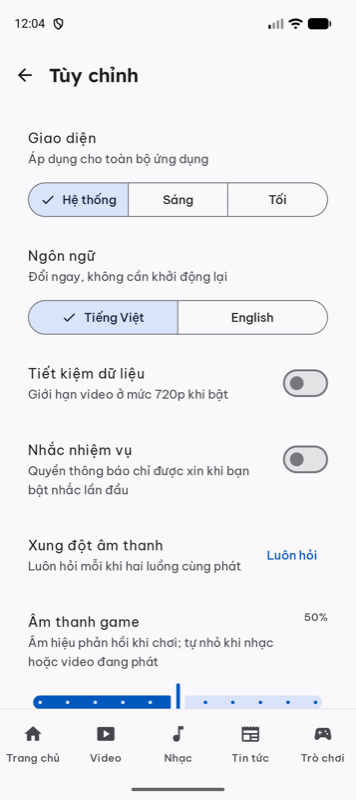
\includegraphics[height=6.1cm]{figures/app/F-GAME-13-01.png}
\end{column}
\end{columns}
\end{frame}

\begin{frame}{Mock Up: Dùng chung}
\begin{columns}[T]
\begin{column}{0.46\textwidth}
{\small\bfseries\color{BKTemplate} F-COM-01: Đăng ký/đăng nhập một tài khoản cho cả 4 phân hệ}\\[2.5mm]
Tính năng thuộc nhóm Major Projects
\end{column}
\begin{column}{0.50\textwidth}
\centering
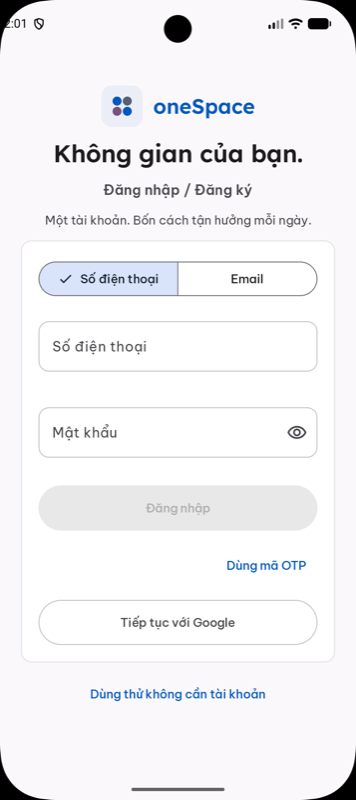
\includegraphics[width=2.32cm]{../figures/app/F-COM-01-01.png}\hspace{0.2cm}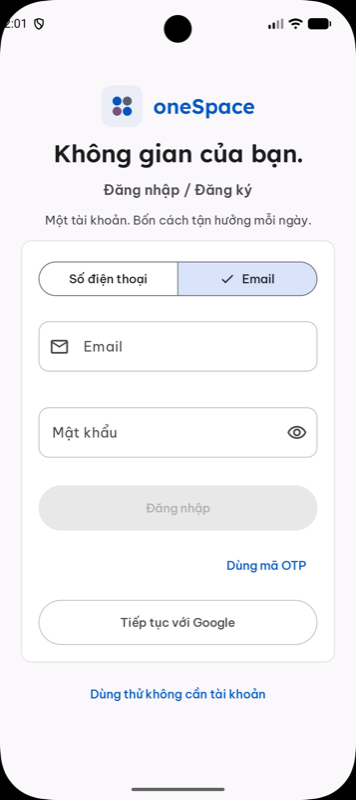
\includegraphics[width=2.32cm]{../figures/app/F-COM-01-02.png}\hspace{0.2cm}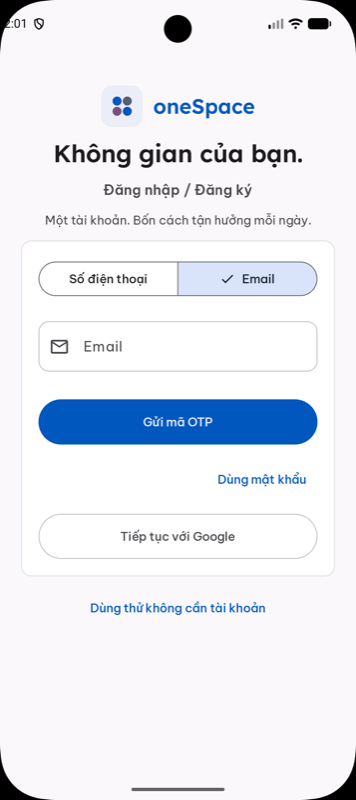
\includegraphics[width=2.32cm]{../figures/app/F-COM-01-03.png}
\end{column}
\end{columns}
\end{frame}

\begin{frame}{Mock Up: Dùng chung}
\begin{columns}[T]
\begin{column}{0.46\textwidth}
{\small\bfseries\color{BKTemplate} F-COM-02: Onboarding chọn sở thích lần đầu}\\[2.5mm]
Tính năng thuộc nhóm Quick Wins
\end{column}
\begin{column}{0.50\textwidth}
\centering
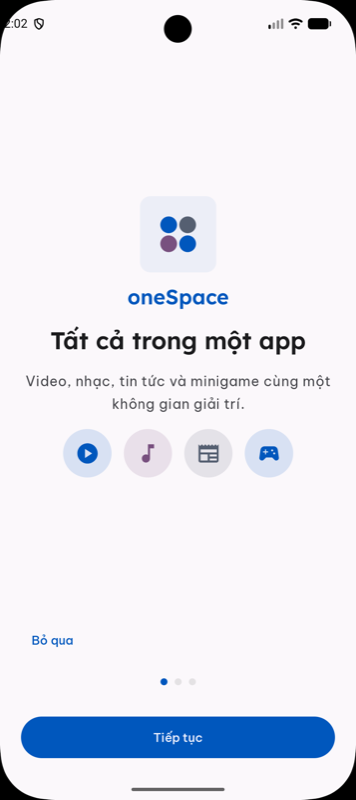
\includegraphics[width=2.32cm]{../figures/app/F-COM-02-01.png}\hspace{0.2cm}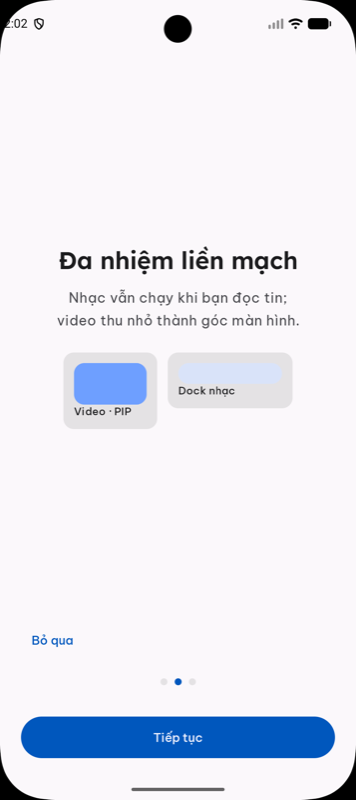
\includegraphics[width=2.32cm]{../figures/app/F-COM-02-02.png}\hspace{0.2cm}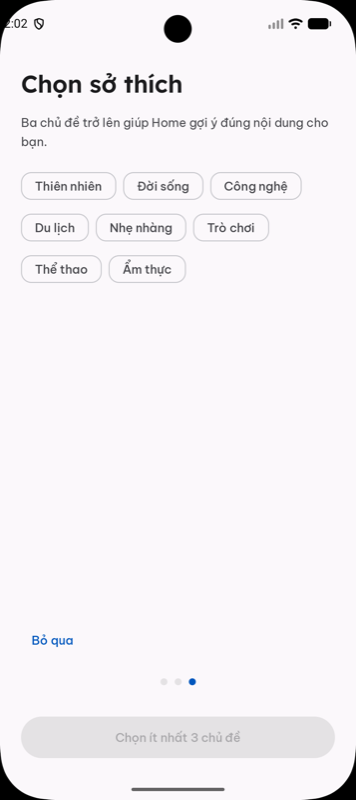
\includegraphics[width=2.32cm]{../figures/app/F-COM-02-03.png}
\end{column}
\end{columns}
\end{frame}

\begin{frame}{Mock Up: Dùng chung}
\begin{columns}[T]
\begin{column}{0.46\textwidth}
{\small\bfseries\color{BKTemplate} F-COM-03: Hồ sơ cá nhân: avatar, khung ảnh theo thành tích}\\[2.5mm]
Tính năng thuộc nhóm Fill-ins
\end{column}
\begin{column}{0.50\textwidth}
\centering
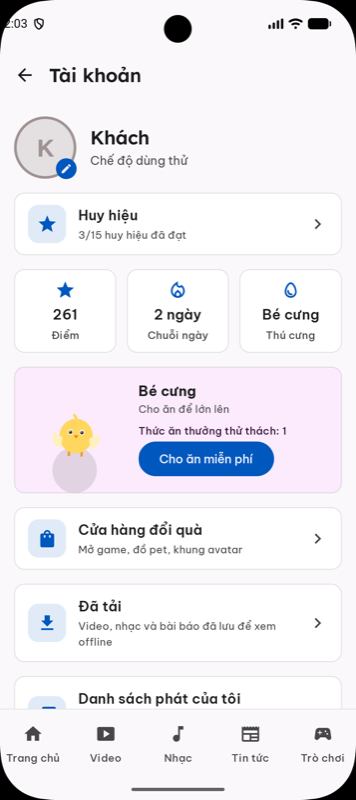
\includegraphics[width=2.75cm]{../figures/app/F-COM-03-01.png}\hspace{0.25cm}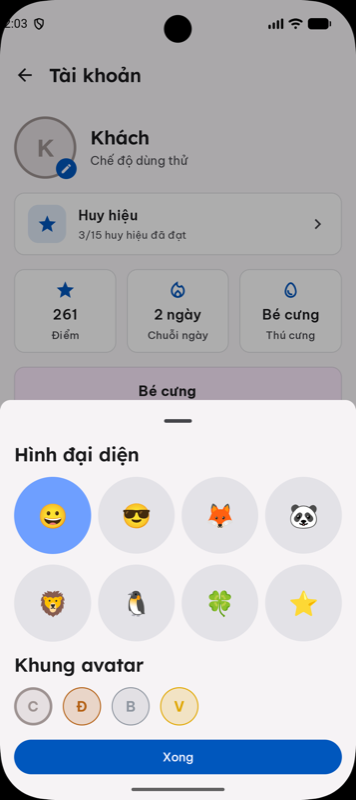
\includegraphics[width=2.75cm]{../figures/app/F-COM-03-02.png}
\end{column}
\end{columns}
\end{frame}

\begin{frame}{Mock Up: Dùng chung}
\begin{columns}[T]
\begin{column}{0.46\textwidth}
{\small\bfseries\color{BKTemplate} F-COM-04: Hệ điểm thưởng dùng chung (XP)}\\[2.5mm]
Tính năng thuộc nhóm Quick Wins
\end{column}
\begin{column}{0.50\textwidth}
\centering
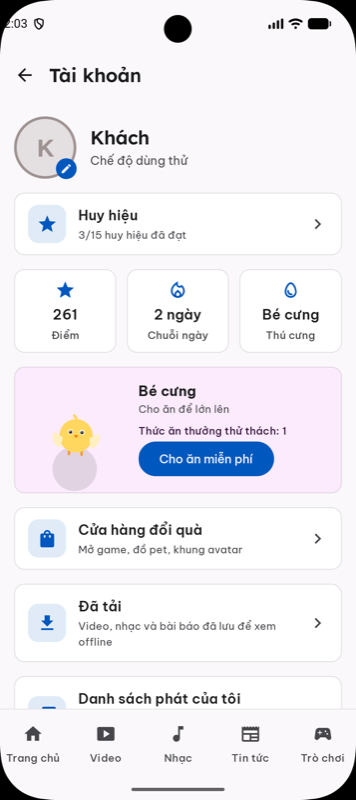
\includegraphics[width=2.75cm]{../figures/app/F-COM-04-01.png}\hspace{0.25cm}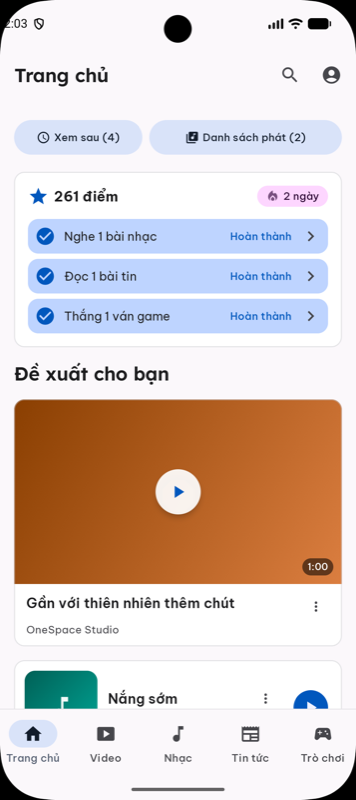
\includegraphics[width=2.75cm]{../figures/app/F-COM-04-02.png}
\end{column}
\end{columns}
\end{frame}

\begin{frame}{Mock Up: Dùng chung}
\begin{columns}[T]
\begin{column}{0.46\textwidth}
{\small\bfseries\color{BKTemplate} F-COM-05: Nhiệm vụ hằng ngày (3--5 nhiệm vụ)}\\[2.5mm]
Tính năng thuộc nhóm Quick Wins
\end{column}
\begin{column}{0.50\textwidth}
\centering
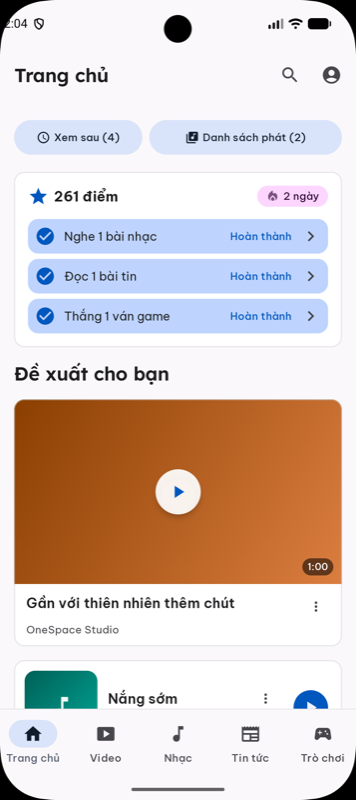
\includegraphics[height=6.1cm]{../figures/app/F-COM-05-01.png}
\end{column}
\end{columns}
\end{frame}

\begin{frame}{Mock Up: Dùng chung}
\begin{columns}[T]
\begin{column}{0.46\textwidth}
{\small\bfseries\color{BKTemplate} F-COM-06: Chuỗi ngày liên tiếp (streak)}\\[2.5mm]
Tính năng thuộc nhóm Quick Wins
\end{column}
\begin{column}{0.50\textwidth}
\centering
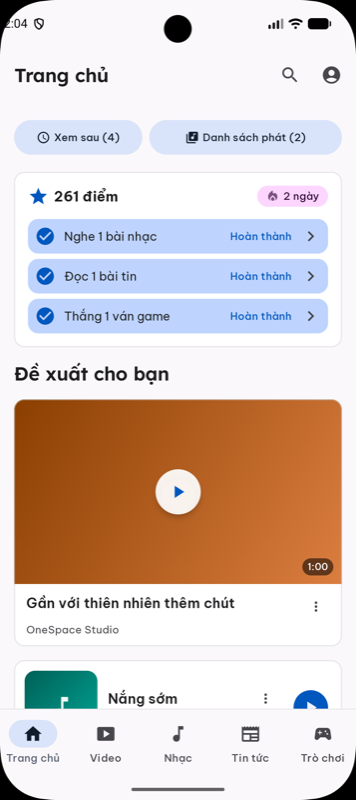
\includegraphics[height=6.1cm]{../figures/app/F-COM-06-01.png}
\end{column}
\end{columns}
\end{frame}

\begin{frame}{Mock Up: Dùng chung}
\begin{columns}[T]
\begin{column}{0.46\textwidth}
{\small\bfseries\color{BKTemplate} F-COM-07: Thú cưng ảo: nuôi bằng điểm, tiến hoá theo mốc}\\[2.5mm]
Tính năng thuộc nhóm Major Projects
\end{column}
\begin{column}{0.50\textwidth}
\centering
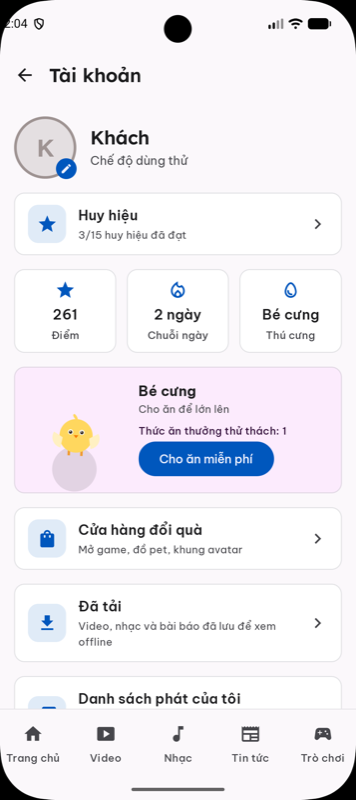
\includegraphics[width=2.75cm]{../figures/app/F-COM-07-01.png}\hspace{0.25cm}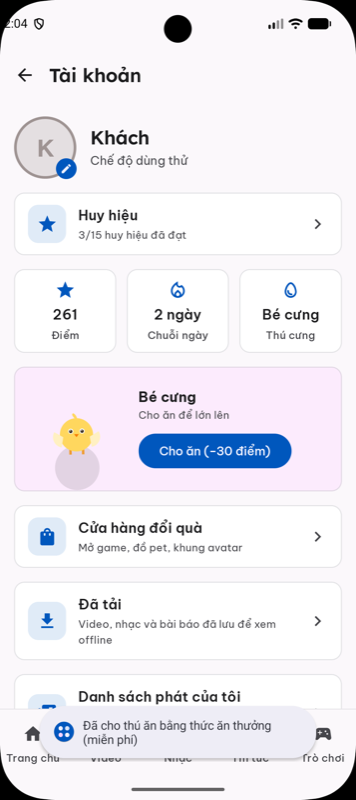
\includegraphics[width=2.75cm]{../figures/app/F-COM-07-02.png}
\end{column}
\end{columns}
\end{frame}

\begin{frame}{Mock Up: Dùng chung}
\begin{columns}[T]
\begin{column}{0.46\textwidth}
{\small\bfseries\color{BKTemplate} F-COM-08: Huy hiệu thành tựu}\\[2.5mm]
Tính năng thuộc nhóm Fill-ins
\end{column}
\begin{column}{0.50\textwidth}
\centering
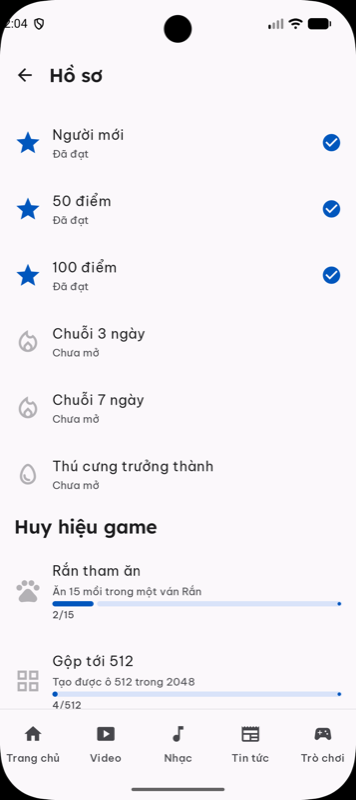
\includegraphics[height=6.1cm]{../figures/app/F-COM-08-01.png}
\end{column}
\end{columns}
\end{frame}

\begin{frame}{Mock Up: Dùng chung}
\begin{columns}[T]
\begin{column}{0.46\textwidth}
{\small\bfseries\color{BKTemplate} F-COM-09: Khung avatar độc quyền theo mốc thành tích}\\[2.5mm]
Tính năng thuộc nhóm Quick Wins
\end{column}
\begin{column}{0.50\textwidth}
\centering
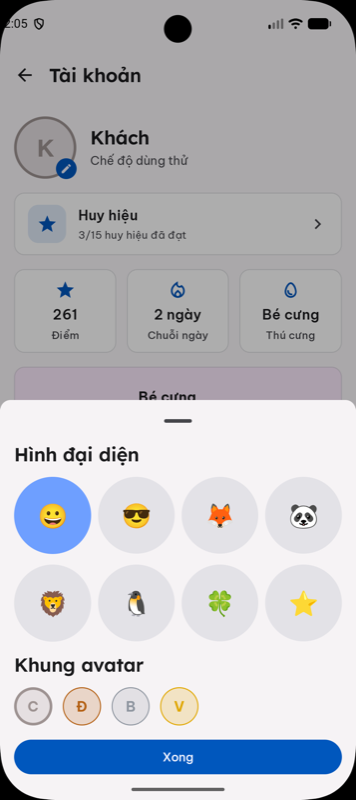
\includegraphics[height=6.1cm]{../figures/app/F-COM-09-01.png}
\end{column}
\end{columns}
\end{frame}

\begin{frame}{Mock Up: Dùng chung}
\begin{columns}[T]
\begin{column}{0.46\textwidth}
{\small\bfseries\color{BKTemplate} F-COM-10: Tổng kết tháng kiểu ``wrapped'', xuất thẻ chia sẻ}\\[2.5mm]
Tính năng thuộc nhóm Major Projects
\end{column}
\begin{column}{0.50\textwidth}
\centering
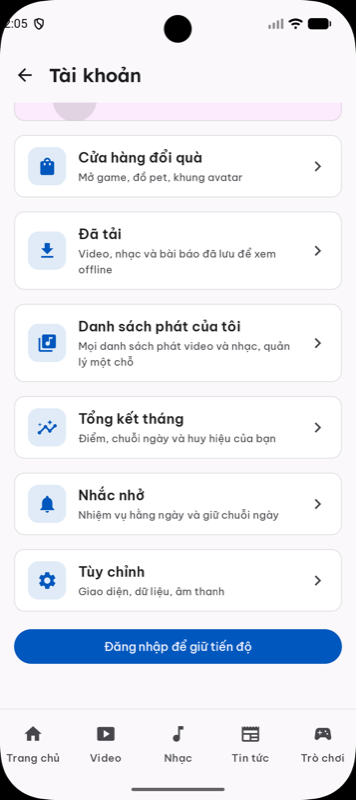
\includegraphics[width=2.32cm]{../figures/app/F-COM-10-01.png}\hspace{0.2cm}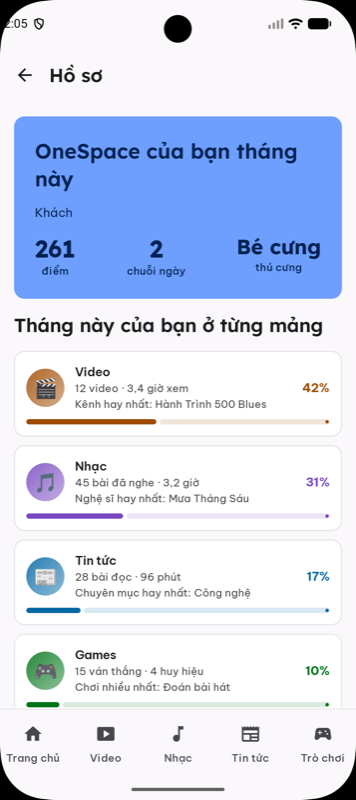
\includegraphics[width=2.32cm]{../figures/app/F-COM-10-02.png}\hspace{0.2cm}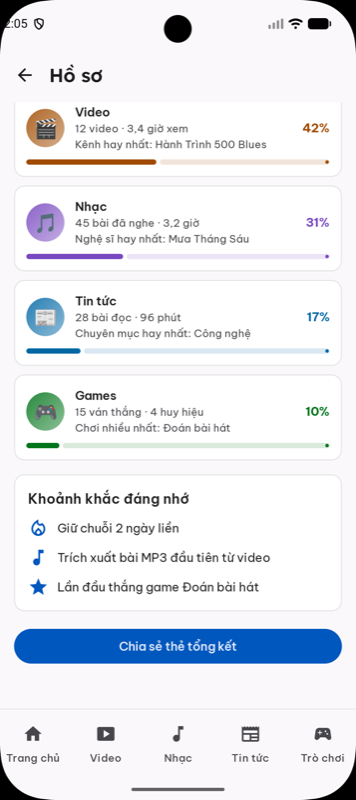
\includegraphics[width=2.32cm]{../figures/app/F-COM-10-03.png}
\end{column}
\end{columns}
\end{frame}

\begin{frame}{Mock Up: Dùng chung}
\begin{columns}[T]
\begin{column}{0.46\textwidth}
{\small\bfseries\color{BKTemplate} F-COM-11: Tìm kiếm xuyên nội dung (một ô tìm cho 4 phân hệ)}\\[2.5mm]
Tính năng thuộc nhóm Major Projects
\end{column}
\begin{column}{0.50\textwidth}
\centering
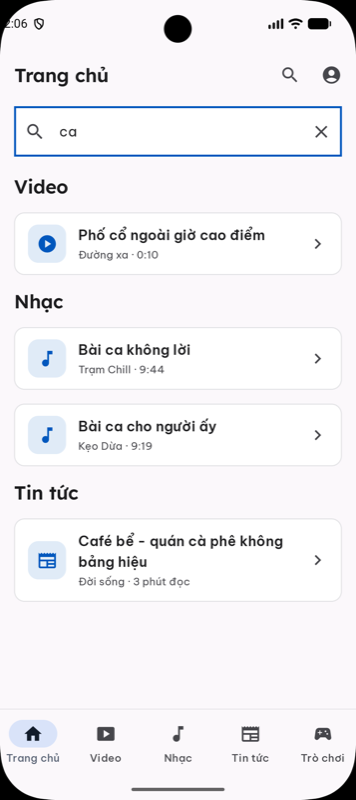
\includegraphics[height=6.1cm]{../figures/app/F-COM-11-01.png}
\end{column}
\end{columns}
\end{frame}

\begin{frame}{Mock Up: Dùng chung}
\begin{columns}[T]
\begin{column}{0.46\textwidth}
{\small\bfseries\color{BKTemplate} F-COM-12: Nhắc nhiệm vụ/streak hằng ngày}\\[2.5mm]
Tính năng thuộc nhóm Quick Wins
\end{column}
\begin{column}{0.50\textwidth}
\centering
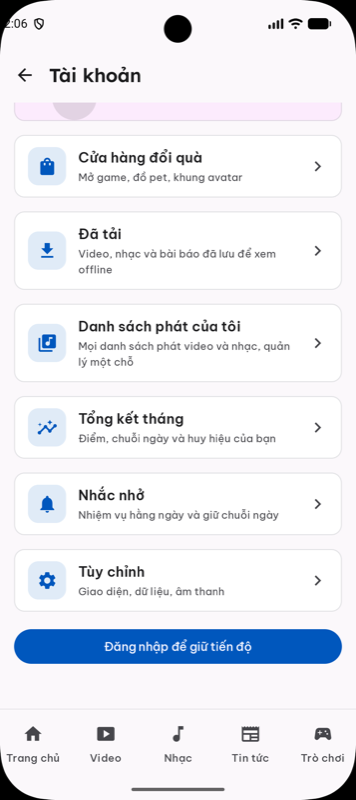
\includegraphics[width=2.75cm]{../figures/app/F-COM-12-01.png}\hspace{0.25cm}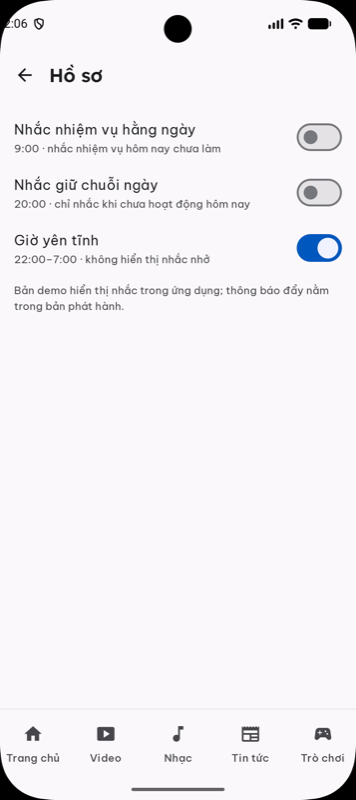
\includegraphics[width=2.75cm]{../figures/app/F-COM-12-02.png}
\end{column}
\end{columns}
\end{frame}

\begin{frame}{Mock Up: Dùng chung}
\begin{columns}[T]
\begin{column}{0.46\textwidth}
{\small\bfseries\color{BKTemplate} F-COM-13: Cài đặt: sáng/tối, ngôn ngữ, tiết kiệm dữ liệu}\\[2.5mm]
Tính năng thuộc nhóm Quick Wins
\end{column}
\begin{column}{0.50\textwidth}
\centering
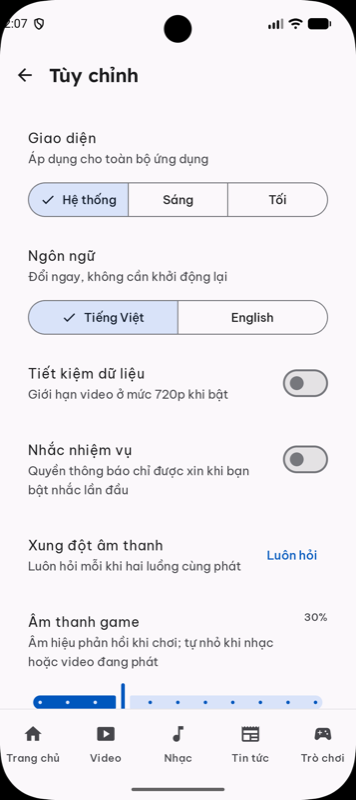
\includegraphics[width=2.75cm]{../figures/app/F-COM-13-01.png}\hspace{0.25cm}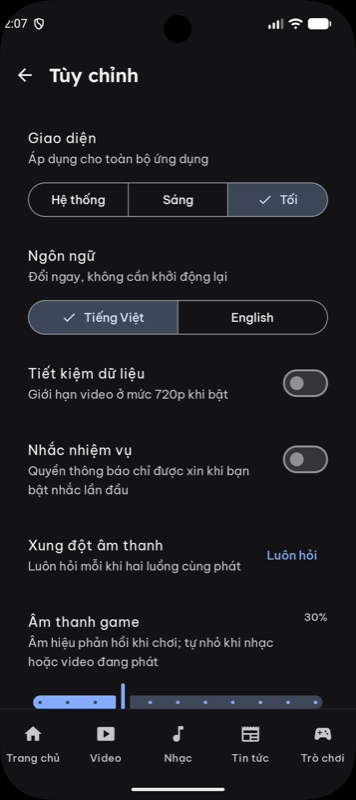
\includegraphics[width=2.75cm]{../figures/app/F-COM-13-02.png}
\end{column}
\end{columns}
\end{frame}

\begin{frame}{Mock Up: Dùng chung}
\begin{columns}[T]
\begin{column}{0.46\textwidth}
{\small\bfseries\color{BKTemplate} F-COM-14: Cửa sổ xác nhận khi hai luồng âm thanh xung đột}\\[2.5mm]
Tính năng thuộc nhóm Quick Wins
\end{column}
\begin{column}{0.50\textwidth}
\centering
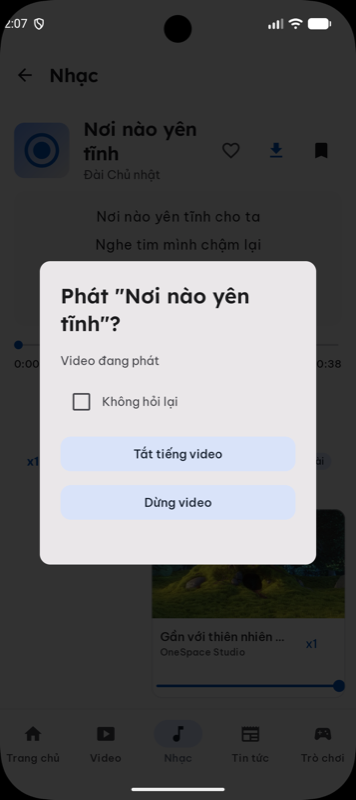
\includegraphics[width=2.75cm]{../figures/app/F-COM-14-01.png}\hspace{0.25cm}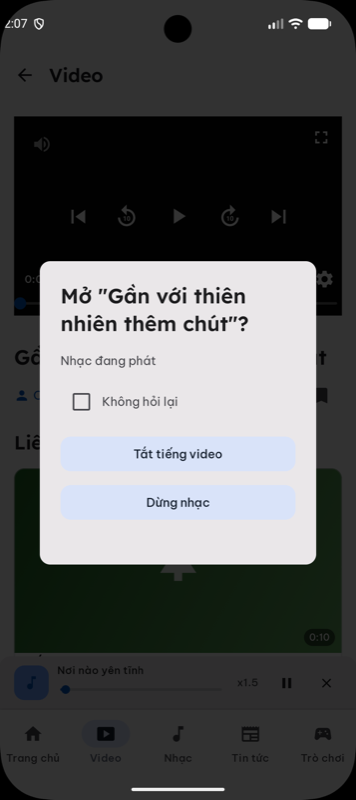
\includegraphics[width=2.75cm]{../figures/app/F-COM-14-02.png}
\end{column}
\end{columns}
\end{frame}

\begin{frame}{Mock Up: Dùng chung}
\begin{columns}[T]
\begin{column}{0.46\textwidth}
{\small\bfseries\color{BKTemplate} F-COM-15: Cửa hàng đổi quà bằng điểm (mở game, đồ pet, khung avatar)}\\[2.5mm]
Tính năng thuộc nhóm Quick Wins
\end{column}
\begin{column}{0.50\textwidth}
\centering
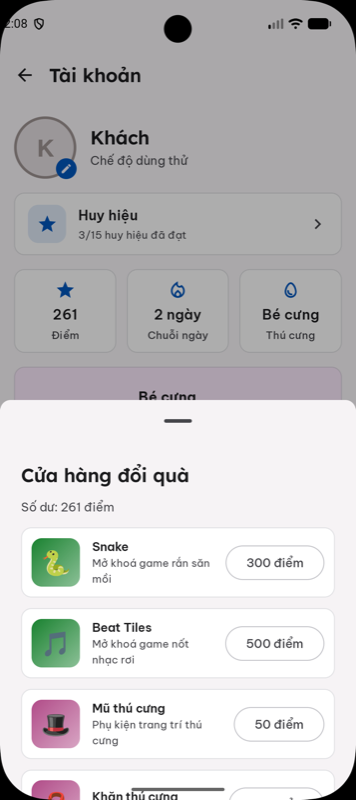
\includegraphics[height=6.1cm]{../figures/app/F-COM-15-01.png}
\end{column}
\end{columns}
\end{frame}

\begin{frame}{Mock Up: Dùng chung}
\begin{columns}[T]
\begin{column}{0.46\textwidth}
{\small\bfseries\color{BKTemplate} F-COM-16: Chế độ ngoại tuyến cơ bản: tin đã lưu, trạng thái mất mạng}\\[2.5mm]
Tính năng thuộc nhóm Major (hoãn tới gần cuối)
\end{column}
\begin{column}{0.50\textwidth}
\centering
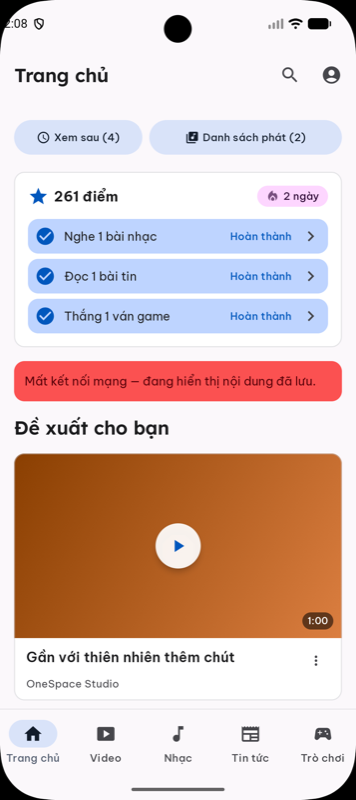
\includegraphics[width=2.75cm]{../figures/app/F-COM-16-01.png}\hspace{0.25cm}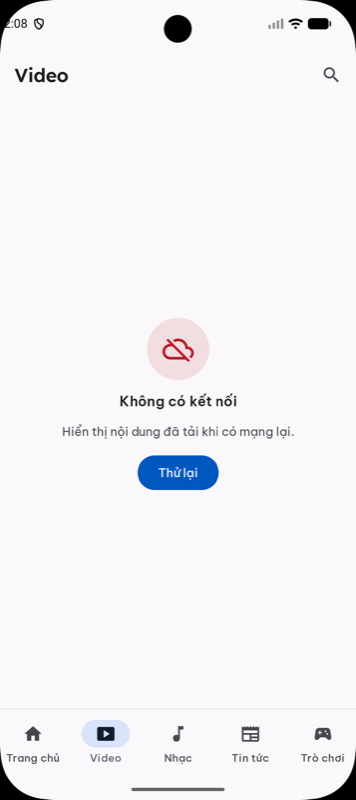
\includegraphics[width=2.75cm]{../figures/app/F-COM-16-02.png}
\end{column}
\end{columns}
\end{frame}

\begin{frame}{Mock Up: Dùng chung}
\begin{columns}[T]
\begin{column}{0.46\textwidth}
{\small\bfseries\color{BKTemplate} F-COM-18: Chế độ khách dùng thử (không cần tài khoản)}\\[2.5mm]
Tính năng thuộc nhóm Quick Wins
\end{column}
\begin{column}{0.50\textwidth}
\centering
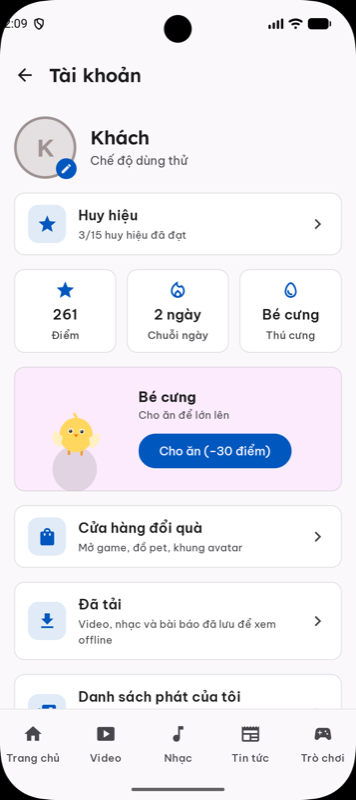
\includegraphics[width=2.75cm]{../figures/app/F-COM-18-01.png}\hspace{0.25cm}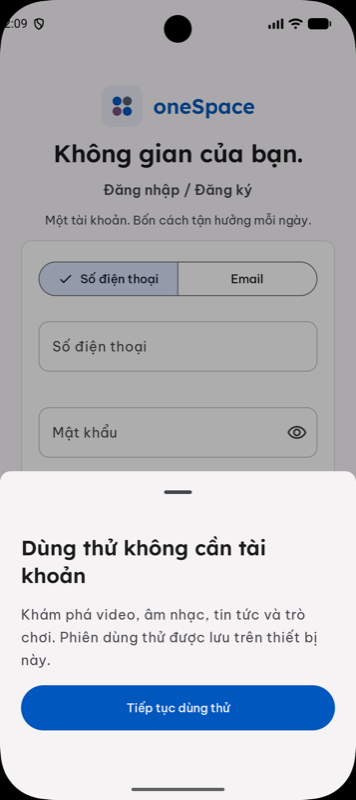
\includegraphics[width=2.75cm]{../figures/app/F-COM-18-02.png}
\end{column}
\end{columns}
\end{frame}

\begin{frame}{Mock Up: Dùng chung}
\begin{columns}[T]
\begin{column}{0.46\textwidth}
{\small\bfseries\color{BKTemplate} F-COM-19: Karaoke/Record: ghi màn hình video (MediaProjection), countdown 3-2-1}\\[2.5mm]
Tính năng thuộc nhóm Major Projects
\end{column}
\begin{column}{0.50\textwidth}
\centering
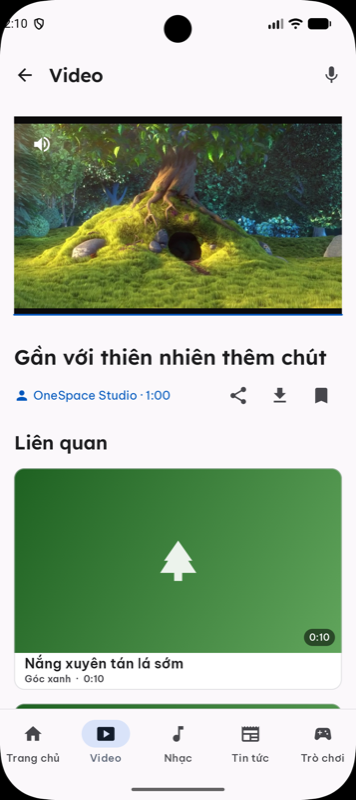
\includegraphics[width=2.32cm]{../figures/app/F-COM-19-01.png}\hspace{0.2cm}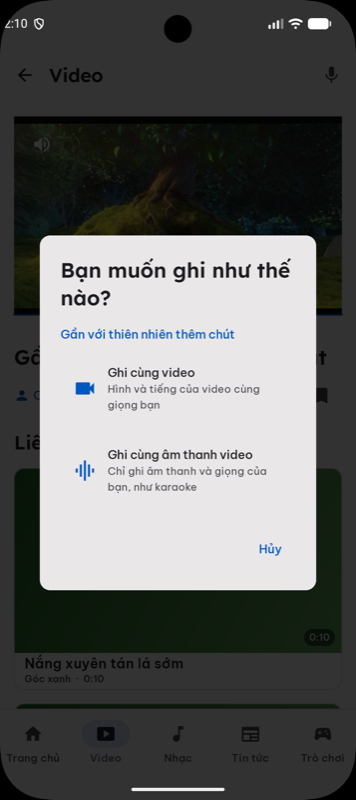
\includegraphics[width=2.32cm]{../figures/app/F-COM-19-02.png}\hspace{0.2cm}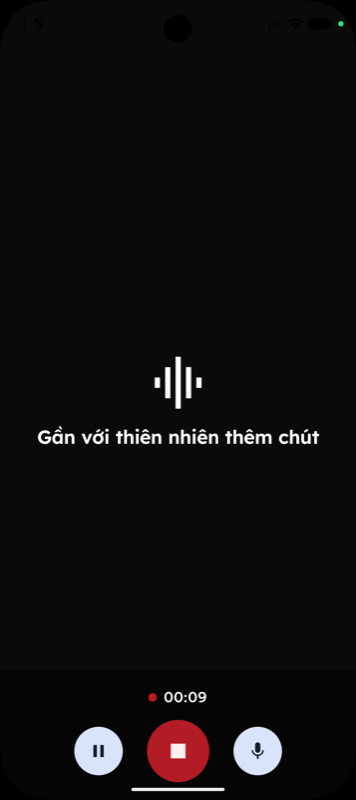
\includegraphics[width=2.32cm]{../figures/app/F-COM-19-03.png}
\end{column}
\end{columns}
\end{frame}

\begin{frame}{Mock Up: Dùng chung}
\begin{columns}[T]
\begin{column}{0.46\textwidth}
{\small\bfseries\color{BKTemplate} F-COM-20: Vuốt ngang đổi phân hệ (trừ Games) + hoàn tác đóng nhạc}\\[2.5mm]
Tính năng thuộc nhóm Quick Wins
\end{column}
\begin{column}{0.50\textwidth}
\centering
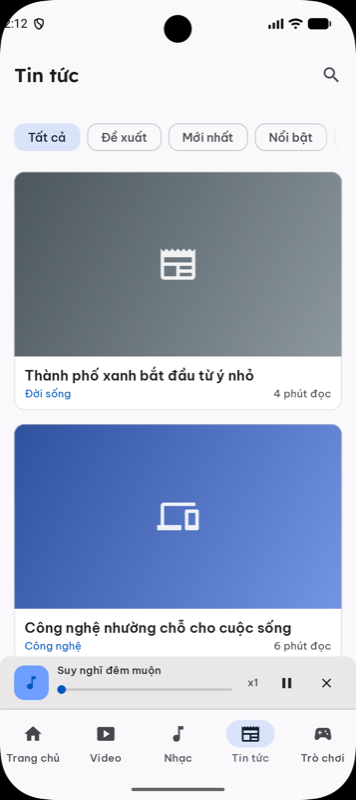
\includegraphics[height=6.1cm]{../figures/app/F-COM-20-01.png}
\end{column}
\end{columns}
\end{frame}

\begin{frame}{Mock Up: Dùng chung}
\begin{columns}[T]
\begin{column}{0.46\textwidth}
{\small\bfseries\color{BKTemplate} F-COM-21: Ghi âm, hát karaoke cùng bài hát đang phát (bên Nhạc)}\\[2.5mm]
Tính năng thuộc nhóm Major Projects
\end{column}
\begin{column}{0.50\textwidth}
\centering
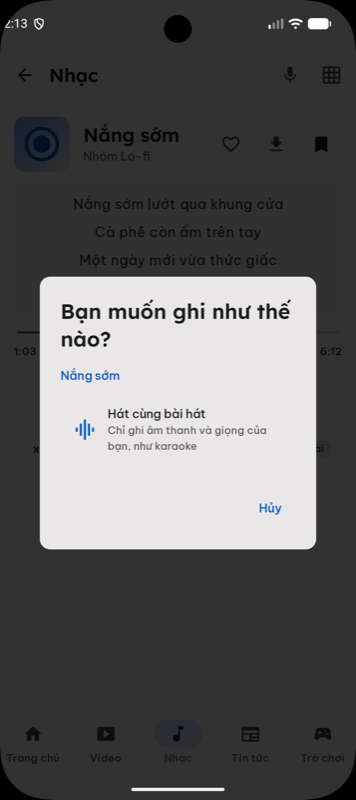
\includegraphics[height=6.1cm]{../figures/app/F-COM-21-01.png}
\end{column}
\end{columns}
\end{frame}

% ===== END MOCKUP =====








\subsection{Design System: Token màu theo vai trò}
% ------------------------------------------------------------
\begin{frame}{Design System --- Token màu theo vai trò}
\begin{columns}[T]
\begin{column}{0.48\textwidth}
{\small\textbf{Màu chính \& nhấn (Light)}}\vspace{1mm}
{\tiny
\begin{itemize}\setlength{\itemsep}{3pt}
\item \sw{0057BD}{F0F2FF} \texttt{primary} 0057BD / dark 85ADFF \newline Nút chính; tab đang chọn; chữ ``Đang phát''; logo
\item \sw{6E9FFF}{001B3F} \texttt{primaryContainer} 6E9FFF \newline Nền icon ContentCard; ô quiz đúng; huy hiệu; nhiệm vụ xong
\item \sw{555F71}{FFFFFF} \texttt{secondary} 555F71 / BDC7DC \newline Icon onboarding; màu phụ logo
\item \sw{78507F}{FFFFFF} \texttt{tertiary} 78507F / E7B6EC \newline Icon streak; nhãn ``Đã xem đến''
\item \sw{FDD6FF}{5E3966} \texttt{tertiaryContainer} FDD6FF / 5E3966 \newline Chip chuỗi ngày; card thú cưng
\item \sw{B31B25}{FFFFFF} \texttt{error} B31B25 / FF716C \newline Lỗi phát; quiz sai; icon yêu thích (tim đỏ)
\end{itemize}}
\end{column}
\begin{column}{0.48\textwidth}
{\small\textbf{Nền, bề mặt \& viền (Light)}}\vspace{1mm}
{\tiny
\begin{itemize}\setlength{\itemsep}{3pt}
\item \sw{FBF8FB}{131315} \texttt{background}/\texttt{surface} FBF8FB / 131315 \newline Nền mọi màn hình; nền card đang kéo (queue)
\item \sw{E3E2E7}{333539} \texttt{surfaceVariant} E3E2E7 / 333539 \newline Ô làn Beat Tiles; nền avatar chưa chọn
\item \sw{EAE7E9}{2A2A2C} \texttt{surfaceContainerHigh} EAE7E9 / 2A2A2C \newline Nền thẻ nổi: banner nhiệm vụ, khung đăng nhập
\item \sw{76777C}{909095} \texttt{outline} 76777C / 909095 \newline Icon radio chưa chọn; vạch phân tách TrackCard
\end{itemize}}
\vspace{1.5mm}
{\tiny
\begin{itemize}\setlength{\itemsep}{3pt}
\item Design system của ứng dụng được xây trên \textbf{Material 3}
\item Mã nguồn không hardcode màu, mọi màn hình đều tham chiếu \textbf{Material Theme}
\end{itemize}}
\end{column}
\end{columns}
\end{frame}

% ------------------------------------------------------------
\subsection{Typography}
% ------------------------------------------------------------
\begin{frame}{Typography --- Nguyên thang chữ Material 3}
\begin{columns}[T]
\begin{column}{0.58\textwidth}
{\tiny\color{TextGray} display $\cdot$ 57sp $\cdot$ splash logo}\\[1pt]
{\fontsize{22}{25}\selectfont\bfseries OneSpace}\\[7pt]
{\tiny\color{TextGray} headline $\cdot$ 24--28sp $\cdot$ tiêu đề màn}\\[1pt]
{\fontsize{14.5}{17}\selectfont\bfseries Thư viện}\\[6pt]
{\tiny\color{TextGray} title $\cdot$ 14--16sp $\cdot$ tiêu đề card, tab}\\[1pt]
{\fontsize{11}{13}\selectfont Nắng sớm}\\[6pt]
{\tiny\color{TextGray} body $\cdot$ 14sp $\cdot$ nội dung, mô tả}\\[1pt]
{\fontsize{9}{11}\selectfont Nhóm Lo-fi $\cdot$ 9:19}\\[6pt]
{\tiny\color{TextGray} label $\cdot$ 11--14sp $\cdot$ chip, nhãn phụ, badge}\\[2pt]
\colorbox[HTML]{E3E2E7}{\textcolor[HTML]{131315}{\fontsize{7.5}{9.5}\selectfont~Tất cả~}}\;\;
{\fontsize{7.5}{9.5}\selectfont\textcolor[HTML]{0057BD}{Đang phát}}\\[9pt]
{\tiny
\begin{itemize}\setlength{\itemsep}{2pt}
\item Nguyên thang M3 (display, headline, title, body, label), không font riêng
\item Đơn vị \texttt{sp} $\rightarrow$ phóng theo cỡ chữ hệ thống
\item Trình đọc bài: riêng 2 nút A$-$/A$+$ (0,8x--1,6x, bước 15\%)
\end{itemize}}
\end{column}
\begin{column}{0.38\textwidth}
\centering
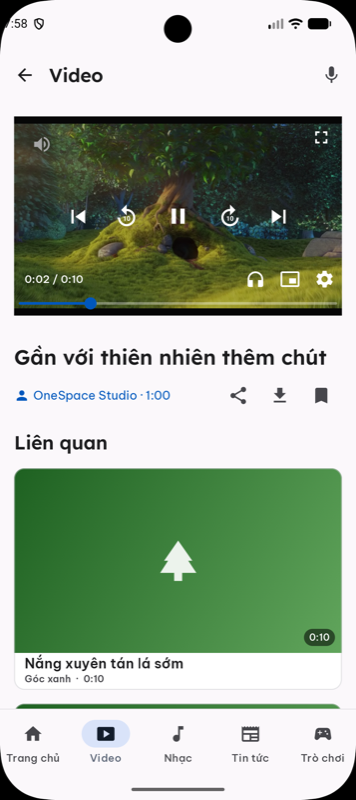
\includegraphics[height=170pt]{../figures/app/F-VID-01-02.png}\\[3pt]
{\tiny\color{TextGray} Màn hình thật}
\end{column}
\end{columns}
\end{frame}

% ------------------------------------------------------------
\subsection{Component}
% ------------------------------------------------------------
\begin{frame}{Component --- Ba nhóm chức năng}
\noindent\begin{minipage}{\textwidth}
{\tiny\color{TextGray} Input control $\cdot$ Navigation $\cdot$ Information --- ảnh chụp từ ứng dụng OneSpace}
\end{minipage}\vspace{2mm}

\begin{columns}[T]
\begin{column}{0.31\textwidth}
\centering
{\small\textbf{1. Input control}}\\[1.5mm]
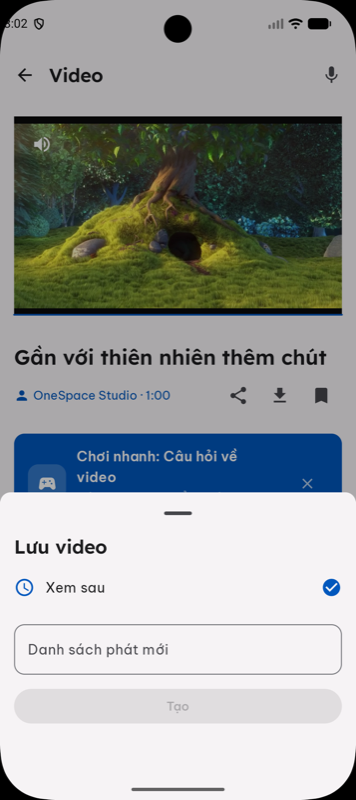
\includegraphics[height=88pt]{../figures/app/F-VID-04-01.png}\\[1.5mm]
{\tiny\color{TextGray} Bảng cài đặt trình phát}\\[1mm]
{\tiny
\begin{itemize}\setlength{\itemsep}{2pt}
\item Ô OTP / mật khẩu
\item Thanh trượt: tốc độ 0,5--2x, âm lượng
\item Chip chất lượng: Auto / 1080p / 720p / 360p
\item Ô tick ``Không hỏi lại''
\end{itemize}}
\end{column}
\begin{column}{0.31\textwidth}
\centering
{\small\textbf{2. Navigation}}\\[1.5mm]
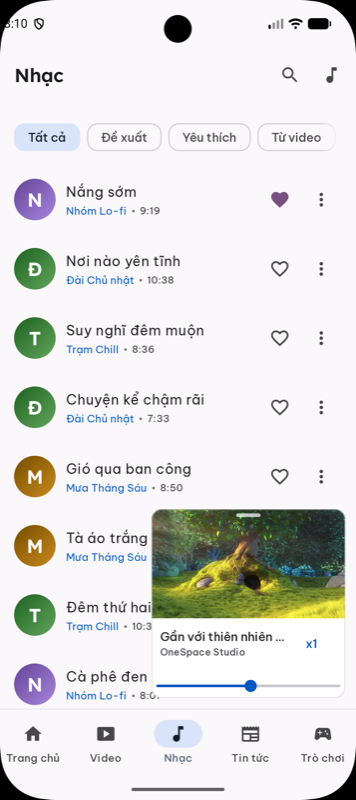
\includegraphics[height=88pt]{../figures/app/F-VID-08-01.png}\\[1.5mm]
{\tiny\color{TextGray} Màn Home --- thanh tab dưới đáy}\\[1mm]
{\tiny
\begin{itemize}\setlength{\itemsep}{2pt}
\item Bottom Nav 5 tab
\item Vuốt ngang đổi phân hệ
\item Nút Quay lại
\item Kéo dock nhạc lên mở hàng đợi
\end{itemize}}
\end{column}
\begin{column}{0.31\textwidth}
\centering
{\small\textbf{3. Information / Container}}\\[1.5mm]
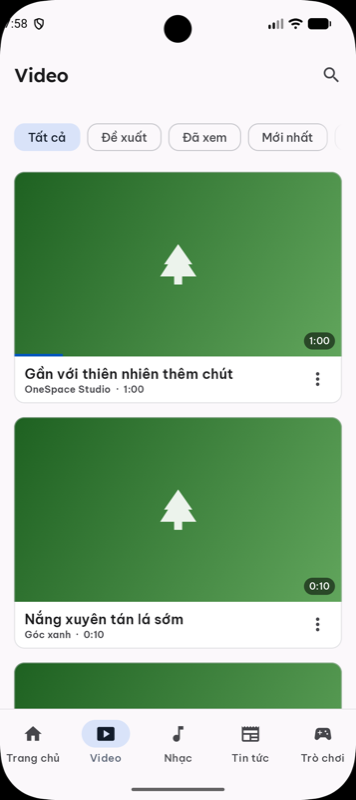
\includegraphics[height=88pt]{../figures/app/F-VID-01-01.png}\\[1.5mm]
{\tiny\color{TextGray} Feed Video --- thẻ nội dung dùng chung}\\[1mm]
{\tiny
\begin{itemize}\setlength{\itemsep}{2pt}
\item ContentCard (thẻ 4 phân hệ)
\item Skeleton feed khi tải
\item Snackbar thông báo
\item Modal Bottom Sheet (hàng đợi, chọn khung)
\end{itemize}}
\end{column}
\end{columns}
\vspace{1.5mm}
{\tiny\textbf{Thư viện dùng chung} (module \texttt{design system}): \texttt{FeaturePage} $\cdot$ \texttt{SectionTitle} $\cdot$ \texttt{ContentCard} $\cdot$ \texttt{CatalogContent} $\cdot$ \texttt{SkeletonFeed} $\cdot$ \texttt{EmptyState}}
\end{frame}

% ------------------------------------------------------------
\subsection{Trạng thái phụ}
% ------------------------------------------------------------
\begin{frame}{Trạng thái phụ: đang tải, trống, lỗi, ngoại tuyến}
\begin{columns}[T]
\begin{column}{0.55\textwidth}
{\small\textbf{Mọi feed dùng chung một bộ chuyển trạng thái}}\\[1.5mm]
{\footnotesize
\begin{itemize}\setlength{\itemsep}{4pt}
\item \textbf{Đang tải:} skeleton 4 hàng + hiệu ứng shimmer, không spinner toàn màn
\item \textbf{Trống:} icon + thông điệp + nút hành động (EmptyState)
\item \textbf{Lỗi:} ``Không tải được'' + nút ``Thử lại'' ở giữa màn hình
\item \textbf{Mất mạng:} banner ``Mất kết nối'' trên Home, nội dung đã lưu vẫn đọc được; có mạng tự phục hồi
\item Ván game cục bộ vẫn chơi được khi offline
\end{itemize}}
\end{column}
\begin{column}{0.41\textwidth}
\centering
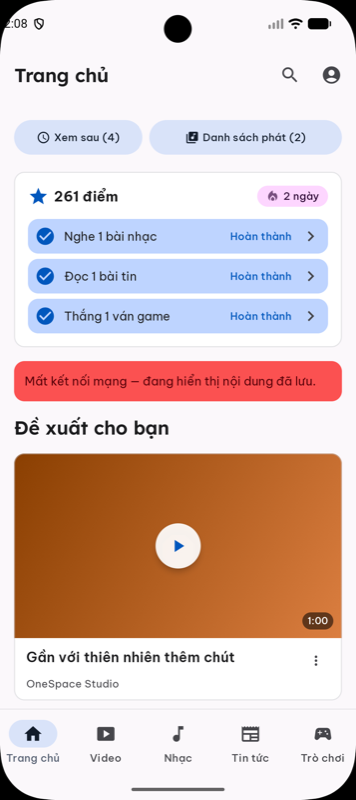
\includegraphics[height=4.1cm]{../figures/app/F-COM-16-01.png}\hspace{1mm}
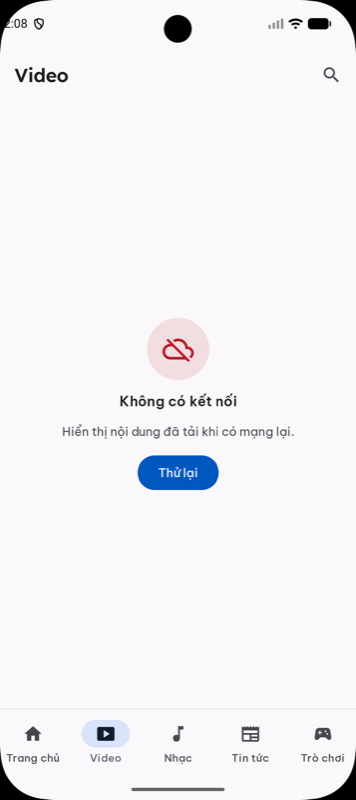
\includegraphics[height=4.1cm]{../figures/app/F-COM-16-02.png}\hspace{1mm}
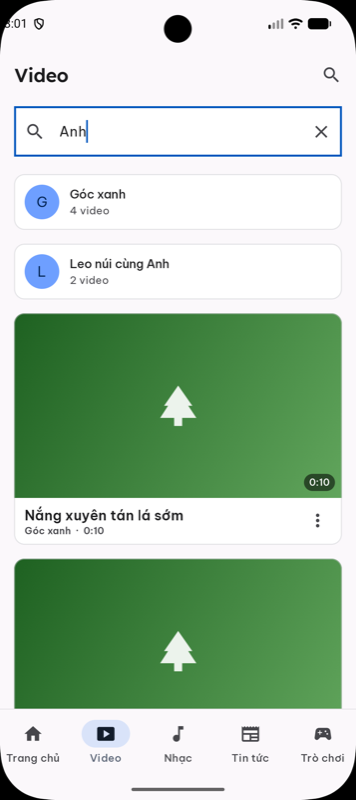
\includegraphics[height=4.1cm]{../figures/app/F-VID-03-02.png}\\[1mm]
{\tiny\color{TextGray} Trạng thái mất mạng (F-COM-16) $\cdot$ tìm kiếm không có kết quả (F-VID-03)}
\end{column}
\end{columns}
\end{frame}

% ------------------------------------------------------------
\subsection{Accessibility}
% ------------------------------------------------------------
\begin{frame}{Accessibility}
\begin{columns}[T]
\begin{column}{0.48\textwidth}
{\small\textbf{Vùng chạm $\geq$ 48$\times$48 dp}}\vspace{1mm}
{\tiny
\begin{itemize}\setlength{\itemsep}{2pt}
\item Mọi nút dùng component M3 $\rightarrow$ tự kế thừa
\item Thẻ nội dung cao $>$ 48dp
\item Ô bàn chơi 2048: 4$\times$4 ô, mỗi ô $>$ 48dp
\end{itemize}}\vspace{2mm}
{\small\textbf{Tương phản màu (WCAG 2.x)}}\vspace{1mm}
{\tiny
\begin{tabular}{@{}lll@{}}
\toprule
\textbf{Cặp} & \textbf{Light} & \textbf{Dark} \\
\midrule
onBackground/bg & 16,3:1 & 14,4:1 \\
onPrimary/primary & 6,4:1 & 7,6:1 \\
onSurfaceVar/surface & 8,9:1 & 10,9:1 \\
outline/bg & 4,3:1 & 5,8:1 \\
\bottomrule
\end{tabular}}
\end{column}
\begin{column}{0.48\textwidth}
{\small\textbf{Ví dụ cặp màu đạt AA}}\vspace{1mm}

\colorbox[HTML]{FBF8FB}{\textcolor[HTML]{131315}{\rule{0pt}{0.28cm}~Nền sáng, chữ tối --- 16,3:1 \textcolor{GreenOK}{\checkmark}~}}\\[3pt]
\colorbox[HTML]{131315}{\textcolor[HTML]{FBF8FB}{\rule{0pt}{0.28cm}~Nền tối, chữ sáng --- 14,4:1 \textcolor{GreenOK}{\checkmark}~}}\\[3pt]
\colorbox[HTML]{0057BD}{\textcolor[HTML]{F0F2FF}{\rule{0pt}{0.28cm}~Nút chính, onPrimary --- 6,4:1 \textcolor{GreenOK}{\checkmark}~}}\\[3pt]
\colorbox[HTML]{B31B25}{\textcolor[HTML]{FFFFFF}{\rule{0pt}{0.28cm}~Nút lỗi, onError --- 6,5:1 \textcolor{GreenOK}{\checkmark}~}}
\vspace{2.5mm}

{\small\textbf{Chữ và trình đọc màn hình}}\vspace{1mm}
{\tiny
\begin{itemize}\setlength{\itemsep}{2pt}
\item Toàn bộ chữ dùng đơn vị sp~--~theo cỡ chữ hệ thống; trình đọc bài có A$-$/A$+$ 0,8x--1,6x
\item TalkBack: nhãn đã thêm ở Account, Nhạc, Tin; thẻ game và một số nút icon chưa đủ~--~tự đánh giá chưa đạt, xếp v2
\end{itemize}}
\end{column}
\end{columns}
\end{frame}

% ------------------------------------------------------------
\subsection{Micro-interactions}
% ------------------------------------------------------------
\begin{frame}{Micro-interactions --- Mô hình Saffer 4 thành phần}
\begin{center}
\begin{tikzpicture}[
    font=\scriptsize,
    comp/.style={draw=BKTemplate, thick, rounded corners=3pt, fill=BKTemplate!8, minimum height=10mm, minimum width=2.4cm, align=center},
    arrow/.style={-{Latex[length=2mm]}, BKTemplate!60, thick}]
  \node[comp] (trg) at (0,0) {\textbf{Trigger}\\Người dùng làm gì};
  \node[comp, right=1.5cm of trg] (rul) {\textbf{Rules}\\Điều kiện áp};
  \node[comp, right=1.5cm of rul] (fdb) {\textbf{Feedback}\\Người dùng thấy gì};
  \node[comp, below=1.2cm of fdb] (lp) {\textbf{Loops \& Modes}\\Hành vi lặp / giới hạn};
  \draw[arrow] (trg) -- (rul);
  \draw[arrow] (rul) -- (fdb);
  \draw[arrow] (fdb) -- (lp);
  \draw[arrow] (lp.west) -- ++(-8.1,0) -- ++(0,3.2) -- (0,0.98) -- (trg.north);
\end{tikzpicture}
\end{center}
\end{frame}

\begin{frame}{Micro-interactions --- Các tương tác đã cài}
\begin{columns}[T]
\begin{column}{0.48\textwidth}
{\scriptsize\textbf{Tải và điều hướng}}\vspace{1mm}
{\tiny
\begin{itemize}\setlength{\itemsep}{2.5pt}
\item \textbf{Skeleton feed:} vào feed khi dữ liệu đang tải, bốn hàng khung xám kèm hiệu ứng shimmer; khung biến mất ngay khi có dữ liệu
\item \textbf{Ripple Material:} mọi nút, thẻ, tab phản hồi bằng vòng sóng lan từ điểm chạm; mặc định toàn hệ thống
\item \textbf{Vuốt ngang:} vuốt trái/phải trên màn feed chuyển sang phân hệ kế bên, giữ nguyên trạng thái từng phân hệ; tắt trong game vì cử chỉ dành cho điều khiển ván chơi
\item \textbf{Dock mini player:} bài đang phát hiện một hàng dock ở đáy mọi màn (kể cả trình đọc bài); chạm mở trình phát đầy đủ
\item \textbf{Cửa sổ nổi:} rời tab khi video đang phát, video thu nhỏ thành cửa sổ ở góc kèm nhãn ``Đang phát'' và ba nút Mở rộng, Tạm dừng, Đóng
\end{itemize}}
\end{column}
\begin{column}{0.48\textwidth}
{\scriptsize\textbf{Tương tác nội dung}}\vspace{1mm}
{\tiny
\begin{itemize}\setlength{\itemsep}{2.5pt}
\item \textbf{Popup C1:} mở nhạc khi video đang phát: hộp thoại hai lựa chọn kèm ô tick ``Không hỏi lại''; không có nút bỏ qua, phải chọn một
\item \textbf{Trạng thái rỗng:} danh mục không có nội dung hiển thị biểu tượng, thông điệp và nút hành động; không để màn hình trống không lối đi
\item \textbf{Mất mạng:} feed không tải được hiện ``Không có kết nối'' kèm nút ``Thử lại''; khi có mạng tự phục hồi
\item \textbf{Bàn chơi 2048:} ô cùng giá trị gộp nhau theo hướng vuốt, bàn chơi và điểm cập nhật tức thì sau mỗi nước
\item \textbf{Beat Tiles:} nốt rơi bốn làn, chạm đúng ô khi nốt vào vùng sáng; điểm và combo tăng tức thì, nhạc vẫn phát
\end{itemize}}
\end{column}
\end{columns}
\end{frame}
